% Class options:
% 3 font choices currently:
%  - Times New Roman (default)
%  - Palantino ('palantino')
%  - Bookman ('bookman')
% Dissertation or Thesis:
%  - Thesis (default)
%  - Dissertation ('dissertation')
% Include bookmarks in compilied pdf
%  - No bookmarks (default)
%  - Bookmarks ('bookmarks')

%\documentclass[dissertation, bookmarks]{grizz_thesis}

\documentclass[thesis, bookmarks]{grizz_thesis}

% Uncomment this to only compile a subset of the document.  List each of the separate include
% files with a comma
%\includeonly{front_matter, chapter1, chapter2}

% Add extra packages here
%\usepackage{someotherpackage}
\usepackage{cases} % allows subnumbers for pieceise functions. 1a,1b
\usepackage{color}					%allows text to have colors
\usepackage{siunitx} % This package is very useful for correct typesetting of numbers and units.
%\usepackage{csquotes} %signle space block quotes 
\usepackage{xcolor,soul}
\usepackage{ragged2e}


%\usepackage[none]{hyphenat}
%\usepackage{lipsum}
%\textwidth=5.70in
%\def\beg{\begin{equation}} 
%%\def\eeg{\end{equation}}
%\def\beq{\begin{equation}} 
%\def\eeq{\end{equation}}
%\def\eeqc{\, , \end{equation}}
%\def\eeqp{\, . \end{equation}}

%\def\crr{\color{red}}
%\def\cbb{\color{black}}

%\usepackage{OUvar} % contains all the variables in the thesis
%\usepackage{physics}

\usepackage{etoolbox}
\AtBeginEnvironment{quote}{\singlespacing\small}


\usepackage{bigints}

% Makes the square root sign cooler
%\usepackage{letltxmacro}
%\makeatletter
%\let\oldr@@t\r@@t
%\def\r@@t#1#2{%
%\setbox0=\hbox{$\oldr@@t#1{#2\,}$}\dimen0=\ht0
%\advance\dimen0-0.4\ht0
%\setbox2=\hbox{\vrule height\ht0 depth -\dimen0}%
%{\box0\lower0.4pt\box2}}
%\LetLtxMacro{\oldsqrt}{\sqrt}
%\renewcommand*{\sqrt}[2][\ ]{\oldsqrt[#1]{#2}}
%\makeatother

  

%allows mathematica code

%\usepackage{listings,xcolor}
%\lstset{language=Mathematica}
%\lstset{basicstyle={\sffamily\footnotesize},
%  numbers=left,
%  numberstyle=\tiny\color{gray},
%  numbersep=5pt,
%  breaklines=true,
%  captionpos={t},
%  frame={lines},
%  rulecolor=\color{black},
%  framerule=0pt,
%  columns=flexible,
%  tabsize=2
%}

%\let\firstchar\lowercase
%\let\oldprintglossaries\printglossaries
%\def\printglossaries{\let\firstchar\uppercase\oldprintglossaries} %This helps the capitalizaiton between akronym list and in text. from  https://tex.stackexchange.com/questions/79907/howto-achieve-capitalized-description-in-glossary-table

%makes equations have parens  %commented out on Jan 20; not sure what changed
%\def\equationautorefname~#1\null{%
  %Equation~(#1)\null}
	
%%%%%%%% Commented out on Jan 20 2020; it changed from (6.7)a to (6.7a) in the site of the equation, and to Equation 6.7a in the text.
%\makeatletter  %This turns the equations into Equation () from https://tex.stackexchange.com/questions/191376/autoref-and-braces-around-equation-number July 21 19
%\let\oldtheequation\theequation
%\renewcommand\tagform@[1]{\maketag@@@{\ignorespaces#1\unskip\@@italiccorr}}
%\renewcommand\theequation{(\oldtheequation)}
%\makeatother

    % First, save the current form of `\theequation`
%    \let\oldtheequation\theequation
%    \makeatletter
%    \def\tagform@#1{\maketag@@@{\ignorespaces#1\unskip\@@italiccorr}}
%    \renewcommand{\theequation}{(\oldtheequation)}
%    \makeatother 
		
		
%\renewcommand{\equationautorefname}{Eq.}  % This changes it from Equation () to Eq. ()

% Uncomment this to force a particular year in the preliminary pages
% If left commented out, the current year will be used instead
%\year=2015

\usepackage{multicol} % added 12/18/2019

% Define custom macros here
\def\ihat{\hat{\imath}}
\def\jhat{\hat{\jmath}}
\def\khat{\hat{k}}

% Add all abbreviations here - Necessary for LIST OF ABBREVIATIONS
% This acronym is not referenced at all and doesn't show up in the LIST OF ABBREVIATIONS
%\newacronym{amcl}{AMCL}{Advanced Monte Carlo Localization} 

\sethlcolor{lightgray}

\begin{document}
\def\thesistitle{On the Relation of Sentiment With Difficulty and Popularity in Stackoverflow}
\def\studentname{Srilakshmi Sripathi}
\def\degreename{Master of Science in Computer Science}
\def\CommitteeChair{Dr. Mehdi Bagherzadeh}
\def\AdvisorOne{Dr. Debatosh Debnath}
\def\AdvisorTwo{Dr. Hua Ming}

%\lipsum[1-50]



%%% Start preliminary pages 
%------------------------------------------
% Formatting code -- DO NOT EDIT
%------------------------------------------
\singlespacing
\pagenumbering{roman}
\titleformat
	{\chapter}
	[display]
	{\normalfont\filcenter\singlespacing}
	{}
	{0pc}
	{#1}
	[\vspace*{3pc}]
%------------------------------------------

%\GrizzCoverPage
\GrizzTitlePage
\GrizzCopyrightPage
\GrizzDedicationPage
\GrizzAcknowledgementsPage
\GrizzAbstractPage
\begingroup
\pagestyle{tocstyle}
\makeatletter
\let\ps@plain\ps@normal
\makeatother
\renewcommand{\contentsname}{TABLE OF CONTENTS}
\ifbookmarks
	\newpage
	\pdfbookmark[0]{\contentsname}{toc}	
\fi

\tableofcontents
\cleardoublepage
\addtolength{\textheight}{0.85in}
\newpage
\endgroup

\phantomsection
\addcontentsline{toc}{chapter}{LIST OF TABLES}	
\begingroup
\pagestyle{lotstyle}
\makeatletter
\let\ps@plain\ps@normal
\makeatother
\listoftables
\cleardoublepage
\addtolength{\textheight}{0.85in}
\newpage
\endgroup

\phantomsection
\addcontentsline{toc}{chapter}{LIST OF FIGURES}
\begingroup
\pagestyle{lofstyle}
\makeatletter
\let\ps@plain\ps@normal
\makeatother
\listoffigures
\cleardoublepage
\addtolength{\textheight}{0.85in}
\newpage
\endgroup

% \phantomsection
% \addcontentsline{toc}{chapter}{LIST OF ABBREVIATIONS}
% %\vspace{0.07in}
% \printglossary[style=grizz_glossary]

%%% Start main body
%------------------------------------------
% Formatting code -- DO NOT EDIT
%------------------------------------------
\pagenumbering{gobble}
\pagenumbering{arabic}
%\newpage
%\begin{center}
%\begin{center}

%\end{center}
%\end{center}
\titleformat
	{\chapter}
	[display]
	{\normalfont\filcenter\singlespacing}
	{\vspace{0.15in}\MakeUppercase{\chaptertitlename~\thechapter}}
	{1pc}
	{#1}
	[\vspace*{2pc}]
\doublespacing

% Equation spacing - adjust if necessary
\setlength{\abovedisplayskip}{0.5pc}
\setlength{\belowdisplayskip}{0.5pc}
\setlength{\abovedisplayshortskip}{0pc}
\setlength{\belowdisplayshortskip}{0.5pc}
%------------------------------------------

% Include each separate chapter source file here
%Introduction
% 2. INTRODUCTION of the Thesis Template File
%\ch{1}
\chapter{INTRODUCTION}

\begin{center}
``Happy software developers solve problems better'' - Graziotin et al. \cite{graziotin2014happy}
\end{center}

In the current software development environment, a software developer's sentiment towards a task may have an impact on their productivity and the overall quality of the software they develop. Understanding this role of the sentiment can help developers and research communities to help in the improvement of the developer's overall throughput.

For the last three decades, improving software quality and software developers' productivity has been a focus; amongst different factors, the people factor has been conside- red one of the vital factors \cite{graziotin2014happy, boehm1988understanding}. So, in recent years, the software engineering community has been focused on software developer's sentiment, as human emotions are volatile and can have a direct impact on their productivity. For instance, developers with a positive sentiment are more likely to be creative and have better analytical problem-solving skills, as illustrated by Graziotin et al. \cite{graziotin2014happy}. While software developers with positive sentiment can be more productive, people with negative sentiment are likely to depart from the project sooner \cite{garcia2013role}.

Currently, the Stackoverflow \cite{stackoverflow2019} website has 11 million software developers as its participants. The platform has 46 million questions and answers posted by those participants, with an average of 6.8 thousand new questions posted daily, and with 10 million visitors to Stackoverflow a day. To enhance their knowledge, developers ranging from beginners to experts often visit the Stackoverflow website to post questions and receive answers from the subject matter experts in the field. For this reason, Stackoverflow is an excellent resource available to study software developers and the problems they encounter. Stackoverflow users often ask questions about software topics like Software Development, Programming Languages, and more. If a user posts a question that does not associate with Software topics, the questions get redirected by the Stackoverflow platform to the appropriate comm- unity within StackExchange. For instance, if a user posts a question related to the educational topic to the Stackoverflow platform, the question gets redirected to the Academia community, which is a subcommunity of StackExchange.

To understand the role of the software developer's sentiment, we perform sentiment analysis, which is a study of lexicons within a text to determine the subjectivity and polarity. Subjectivity helps determine if the text is emotionally loaded or if it is neutrally toned. On the other hand, polarity checks if the meaning of the text is positive, negative, or neutral. The sentiment for the entire text is determined by analyzing the values for subjectivity and polarity for each lexicon. We are interested in analyzing the role of the sentiment with software topics that are difficult to understand and concepts that are currently popular. 

In this thesis, we conducted a large-scale study on the Stackoverflow questions and answers for big data and concurrency software development. We focused our attention on the software developer's sentiment and its correlations with popularity and difficulty by answering the research questions \emph{\textbf{R1}} to \emph{\textbf{R4}}, as shown below. To perform our analysis, we rely on two previous works on concurrency and big data \cite{ahmed2018concurrency, bagherzadeh2019going}. We considered concurrency topics since developers find it challenging to develop concurrency programs, while big data topics are currently popular concepts. The concurrency dataset \cite{ahmed2018concurrency} has 250K questions and answers with 29 concurrency topics, and the study calculates the difficulty and popularity percentages. Similarly, in the big data dataset, the dataset has 150K questions and answers with 27 big data topics, and the study calculates the difficulty and popularity percentages. 

We study the relationship between sentiment with both popularity and difficulty metrics by computing the sentiment for each topic in the two datasets and find if a correlation exists to understand the following questions:

\emph{\textbf{R1}}. Is there a relation between sentiment with popularity and sentiment with difficulty in concurrency topics?
%\label{textR1}

\emph{\textbf{R2}}. Is there a relation between sentiment with popularity and sentiment with difficulty in big data topics?

\emph{\textbf{R3}}. What sentiment do concurrency and big data developers express towards a common topic?

\emph{\textbf{R4}}. Is there a commonality in the correlations found in concurrency and big data datasets?
 
This thesis's chapters are structured as follows. In Chapter 2, we discuss the dataset, sentiment analysis tool Senti4SD, and finally, we mention the steps we used to perform the analysis. In Chapter 3, we present the results of the sentiment analysis for the concurrency and big data datasets and examine the correlations. In Chapter 4, we present the implications of this study. In Chapter 5, we review works that are related to this study. Finally, we present the conclusion and the future work in Chapter 6.

%Methodology
%\def\L{\textless}
\def\G{\textgreater}
\chapter{METHODOLOGY}

In this chapter, we examine the methods used in our analysis in detail to answer the research questions \emph{\textbf{R1}} to \emph{\textbf{R4}}. We begin with the background of the Stackoverflow questions and answers. Next, our methodology to perform sentiment analysis. Finally, we discuss the methods to find whether correlations exist within the datasets.

\section{Stackoverflow Questions and Answers}
It is essential to understand the structure of Stackoverflow questions and answers and their usage in our analysis. When a registered Stackoverflow participant posts a question related to software topics, the post generates question metadata. Similarly, when a participant answers the posted question, it generates answer metadata. When the participant requesting the question receives a relevant answer, the most relevant answer becomes an accepted answer. The Stackoverflow participant and platform are the two sources that generate the question metadata. The participant generates the question title, descriptive question body, relevant tags, and accepted answer. While the Stackoverflow platform generates the unique identifier, date and time of the post, the number of favorites, score, and the number of views to the question. 

Similarly, the answer metadata has two sources, where the participant generates the answer body, and the platform generates the answer identifier and date. When participants post duplicate questions, the Stackoverflow platform often merges the two questions into one. If a participant considers and marks an answer as a relevant solution for this problem, then the Stackoverflow platform considers that answer as an accepted answer. For an example question and answer metadata, refer to the Table \ref{questions} and the Table \ref{answers} and note the metadata updates with time.

\begin{table}[t!hb]
\caption{Stackoverflow Sample Question}
\label{questions}
% this question has neutral sentiment: positive
\centering
\begin{tabular}{p{1.7in}p{1.5in}p{2.5in}} \hline
\textbf{Question Metadata} & \textbf{Description} & \textbf{Example}\\ \hline
question id & unique identifier & 47613802\\ 
\\
title & title given by user & how to create threads dynamically? \\
\\
body & question content & I want to create certain number of threads in my program where the number of threads to be created is provided by the user at run-time\\
\\
date & time and date of post & 2017-12-02 23:44:13.160\\ 
\\
tags & Stackoverflow tags & multithreading, java, dynamic\\
\\
favorites & count of user likes & 79\\ 
\\
score & like and dislike score & 150\\
\\
views & total views & 454\\
\\
accepted answer & user accepted answer & 47613819 \\ \hline
\end{tabular}
\end{table}


\begin{table}[b!ht]
\caption{Stackoverflow Sample Answer}
\label{answers}
\centering
\begin{tabular}{p{1.7in}p{1.5in}p{2.5in}} \hline
\textbf{Answer Metadata} & \textbf{Description} & \textbf{Example}\\\hline
answer id & a unique identifier & 47613819 \\ 
\\
date & time and date of post & 2017-12-02 23:47:28.157 \\
\\
body & an answer to question & there are a number of ways to do this. A for loop is the easiest your runnable couple be something like this\\ \hline
\end{tabular}
\end{table}


\section{Concurrency and Big Data Datasets}

To perform our sentiment analysis study, we begin by examining the data for concur- rency \cite{ahmed2018concurrency} and big data \cite{bagherzadeh2019going} by using the two datasets from the previous publications. These two papers analyze the Stackoverflow question and answer posts from the Stackoverflow official data dump, which is publicly available at \cite{stackoverflow2019}. In this section, we discuss the contents of the two datasets, as shown in Figure \ref{last}; these are the questions and answers, the topics, and the measures for popularity and difficulty metrics.

\subsection{Concurrency and Big Data Questions and Answers}
\label{dataset}
For concurrency dataset, we utilized Ahmed and Bagherzadeh's work \cite{ahmed2018concurrency}, which analyzes the Stackoverflow data over 9 years from August 2008 until December 2017. This dataset includes 38,485,046 questions and answers posted by 3,589,412 software developer participants of the Stackoverflow platform. Among these posts, 14,995,834 (39\%) are questions and 23,489,212 (61\%) are answers. From 38,485,046 questions and answers, the study concluded by identifying 245,576 (64\%) of questions and answers belonging to the topic of concurrency. In those concurrency posts of the total of 245,576 questions and answers, 156,812 (64\%) belong to question posts and 88,764 (36\%) belonging to answer posts.

To study big data developers, we utilized the data from Bagherzadeh and Khatchad- ourian \cite{bagherzadeh2019going} work, which categorizes Stackoverflow questions and answers as big data topics. The input dataset for the study includes 42,850,541 Stackoverflow questions and answers posted by 4,142,516 software developers over a 10-year duration from August 2008 to December 2018. The study identifying 157,525 questions and answers belonging to big data topics of those, 112,948 (72\%) are questions, and 44,577 (28\%) are answers. Our study aggregates both papers, and our dataset input has 403,413 questions and answers containing 269,818 (67\%) questions and 133,595 (33\%) answers. To see the statistics of our dataset, refer to Table \ref{tabStat}. We perform sentiment analysis on 403,413 questions and answers to answer our research questions.

\subsection{Concurrency and Big Data Topics} 
\label{topicssec}
To study the sentiment of concurrency and big data topics, we utilize the topic categorization conducted by the papers \cite{ahmed2018concurrency, bagherzadeh2019going}. These two works categorize the questions and answers using Latent Dirichlet Allocation (LDA) \cite{blei2003latent} and an open card sort. Topic modeling using LDA means assigning related topic names over a normal distribution based on keywords existing in the question and answer. And, an open card sort means that topic names are not predefined but assigned in the topic labeling process. The topic labeling process the studies \cite{ahmed2018concurrency, bagherzadeh2019going} follow, is that they manually sample through 15 random posts from individual topics. By iteratively refining associated topics, 27 topics names were manually assigned to 245,576 concurrency questions and answers. To see the concurrency topic names and their descriptions, refer to Table \ref{tab:CT}. For 157,525 big data questions and answers, the study \cite{bagherzadeh2019going} assigns them to 28 big data topics. For detailed big data topic names and descriptions, refer to Table \ref{tab:BT}. We perform sentiment analysis to assess sentiments for each topic in concurrency and big data datasets.

\begin{table}[h!bt]
\caption{Statistics of Concurrency and Big Data Dataset}
\label{tabStat}
\centering 
\begin{tabular}{p{.9in}p{1.4in}p{1.4in}p{1.4in}} \hline
\textbf{Dataset} & \textbf{No. of Q\&As} & \textbf{No. of Questions} & \textbf{No. of Answers}\\  \hline
concurrency & 245,576 & 156,812 (64\%) & 88,764 (36\%) \\
\\
big data & 157,525 & 112,948 (72\%) & 44,577 (28\%) \\\hline
\textbf{Total} & \textbf{403,413} & \textbf{269,818 (67\%)} & \textbf{133,595 (33\%)} \\ \hline
\end{tabular}
\end{table}

\begin{table}[tbp]
\caption{Concurrency Topics From the Previous Work \cite{ahmed2018concurrency}}
\centering
\label{tab:CT}
\begin{tabular}{p{.15in}p{2.25in}p{3.1in}}\hline
%\textbf{No.}&\textbf{Topic}&\textbf{Topic Description for Q \& A's }\\ \hline
\textbf{No.}&\textbf{Topic}&\textbf{Q \& As Topic Words}\\ \hline
1&basic concepts & 
code understand read find edit make\\

2&task parallelism & 
task schedul async asynchron parallel\\

3&producer-consumer concurrency & 
queue consum produc process buffer block\\

4&parallel computing & 
parallel node loop comput openmp mpi\\

5&process life cycle management& 
process child parent termin fork kill start\\

6&python multiprocessing& 
python script run multiprocess parallel php\\

7&thread life cycle management& 
thread execut background separ join finish\\

8&thread sharing& 
variabl pass call pointer pthread global\\

9&thread scheduling& 
loop time wait stop run start sleep set check\\

10&thread pool & 
pool job process task limit threadpool\\

11&concurrent collections& 
list arrai map element collect iter kei add\\

12&thread safety& 
thread java safe multipl multi multithread\\

13&locking& 
lock mutex wait condit semaphor acquir\\

14&memory consistency& 
read write variabl atom cach share synchron\\

15&entity management& 
concurr session spring entiti transact actor\\

16&database management systems& 
databas tabl queri row record lock insert sql\\

17&file management& 
file read write log line open stream directori\\

18&object-oriented concurrency& 
object class method creat static access\\

19&web concurrency& 
servic web server applic user app net http\\

20&event-based concurrency& 
event signal handler timer callback call slot\\

21&mobile concurrency& 
android app view updat frame asynctask\\

22&client-server concurrency& 
connect send socket receiv port read\\

23&data scraping& 
data time load download problem\\

24&runtime speedup& 
cpu core time performance\\

25&unexpected output& 
code work run output problem print line\\

26&irreproducible behavior& 
error run problem applic compil crash\\

27&GUI& 
updating gui windows applications\\ \hline
\end{tabular}
\end{table}

\begin{table}[tbp]
\caption{Big Data Topics From the Previous Work \cite{bagherzadeh2019going}}
\centering
\label{tab:BT}
\begin{tabular}{p{.15in}p{2.25in}p{3.1in}}\hline
\textbf{No.}&\textbf{Topic}&\textbf{Q \& As Topic Words}\\ \hline
1&memory management & 
memori executor task job spark run core\\ 

2&PIG& 
pig scripts oozi job workflow action run error\\ 

3&connection& 
connect hadoop server instal cloudera\\ 

4&dataset load\&store & 
file data spark read json csv parquet load\\ 

5&data organization& 
partit join data number case oper kei set\\ 

6&scala spark& 
scala spark org apach java sql appli anonfun\\ 

7&pyspark& 
python pyspark spark zeppelin error run\\ 

8&dataframe& 
column datafram row spark pyspark data\\ 

9&file distribution& 
node hadoop cluster namenod hdf datanod\\

10&general programming& 
class function method object call code type\\ 

11&debugging& 
error code run work problem issu except fail\\ 

12&hbase& 
hbase tabl row region zookeep client scan\\ 

13&job management& 
spark run cluster job applic submit yarn\\ 

14&file format& 
file line read input split text block size data\\

15&file management& 
file hdf directori path hadoop folder local\\ 

16&string& 
string type field arrai null column valu\\ 

17&database import\&export& 
sqoop cassandra jdbc mysql databas connector\\ 

18&stream processing& 
stream spark kafka data messag batch process\\ 

19&basic concepts& 
data hadoop process system databas solut\\ 

20&date\&time& 
date time timestamp data month event record\\ 

21&logging& 
info flume log java org channel apach sink\\ 

22&performance& 
data perform memori process size run million\\ 

23&text search& 
document mongodb queri collect elastic search\\ 

24&dependency management& 
jar hadoop version spark java error run depend\\ 

25&debugging& 
java org apach hadoop lang run mapr util\\ 

26&machine learning& 
model spark vector mahout train featur data\\ 

27&hive analysis& 
hive tabl queri creat data sql select insert\\ 

28&mapreduce& 
kei group count reduc hadoop map reduc\\ 

29&RDD& 
rdd spark transform code function scala map\\ \hline
\end{tabular}
\end{table}

\clearpage
\subsection{Concurrency and Big Data Popularity and Difficulty}
We utilized popularity and difficulty metrics for the concurrency and big data topics from \cite{ahmed2018concurrency, bagherzadeh2019going} to determine the correlation between sentiment with popularity and sentiment with difficulty. The authors evaluated popularity and difficulty metrics using questions and answers metadata of the Stackoverflow, given in Table \ref{questions} and the Table \ref{answers}. The popularity metric was calculated by 3 well-known measures, which are the average views, average favorites, and average scores. Likewise, they evaluated the difficulty metric using 2 well-known measures, which are the percentage of questions without accepted answers and the hours to receive an accepted answer.

To be more specific, the definitions of the popularity metrics are as follows; they defined average views measure \cite{bajaj2014mining, nadi2016jumping, rosen2016mobile, yang2016security} as the average number of visits to the posted question to the number of questions in a topic. They considered the average views measure because Stackoverflow allows both registered and unregistered users to visit questions. We consider average views because the number of views to the Stackoverflow platform by the unregistered users is higher in number compared to registered users \cite{mamykina2011design}. Secondly, as defined in \cite{bajaj2014mining, nadi2016jumping, pinto2015study, yang2016security}, the average favorites measure uses the question metadata’s favorites counter by taking the average of it within a topic. To be more specific, the average favorites is the total number of registered users who mark the question as to their favorites. Finally, as defined in \cite{bajaj2014mining, nadi2016jumping, pinto2015study, yang2016security}, the average scores measure is calculating the average of the question metadata’s scores counter within a topic. To be more specific, the average scores is the total number of registered users who like or dislike the question. For more details about popularity metrics, refer to Table \ref{PM}.

\begin{table}[h!tb]
\caption{Popularity and Difficulty Metrics}
\label{PM}
\centering
\begin{tabular}{p{0.70in}p{1.20in}p{3.60in}} \hline
\textbf{Metrics} & \textbf{Measures} & \textbf{Description}\\ \hline
popularity & average views & an average number of views for all the questions in a topic the questions in a topic \\
\\
& average favorites & total average of users marking the question as their as their favorite in a topic \\
\\
& average scores & average of raw score for all the questions within a topic \\
\\
difficulty & \%w/o acc. answer & percentage of questions without accepted answers \\
\\
& hrs to acc. answer & average median time needed for questions of a topic to receive accepted answers\\ \hline
\end{tabular}
\end{table}

On the other hand, the difficulty metric defined 2 measures that are as follows. The first measure the percentage of questions that do not have accepted answers within a topic \cite{rosen2016mobile, treude2011programmers,yang2016security}. The second measure checks the average time that is taken for a question in a topic to receive an accepted answer \cite{rosen2016mobile, yang2016security}. More straightforward questions tend to receive solutions faster compared to harder questions. Measures of the difficulty metric are in Table \ref{PM}.

The authors in \cite{ahmed2018concurrency, bagherzadeh2019going} calculated popularity and difficulty metrics for concurrency and big data topics using the five measures defined as above. Note, the values calculated for the measures dependent on questions and answers metadata and the time the information is gathered. The values for the popularity and difficulty measures for the concurrency topics are in the Table \ref{CP}. Likewise, the values for these two measures for the big data topics are in Table \ref{BP}.

\begin{table}[tbp]
\caption{Popularity and Difficulty Metrics for the Concurrency Topics From the Previous Work \cite{ahmed2018concurrency}}
\label{CP}
%\begin{tabular}{p{1.5in}p{.6in}p{.6in}p{.6in}p{.7in}p{.6in}} \hline
\begin{tabular}{p{1.7in}p{.5in}p{.6in}p{.4in}p{.9in}p{.9in}} \\ \hline
\textbf{Topic} & \textbf{Popularity} & & & \textbf{Difficulty} \\\hline
& \textbf{Avg. views} & \textbf{Avg. favorites} & \textbf{Avg. scores} & \textbf{\%w/o acc. answer} & \textbf{Hrs to acc. answer}\\ \hline
thread safety & 2848 & 1.5 & 4.6 & 39.6 & 0. 3\\ 
basic concepts & 2222 & 1.6 & 4.3 & 37.0 & 0.7 \\ 
task parallelism & 2216 & 1.3 & 4.0 & 35.3 & 0.4 \\ 
locking & 2152 & 1.3 & 3.5 & 40.1 & 0.3\\ 
thread life cycle management & 2130 & 0.7 & 2.4 & 40.4 & 0.3\\ 
thread scheduling & 2032 & 0.7 & 2.2 & 40.8 & 0.4\\ 
process life cycle management & 2004 & 1.0 & 2.6 & 44.9 & 0.6\\ 
thread pool & 1841 & 0.9 & 2.7 & 47.0 & 0.7\\ 
object-oriented concurrency & 1773 & 0.8 & 2.6 & 35.2 & 0.3\\ 
database management systems & 1727 & 0.6 & 1.8 & 51.2 & 1.0\\ 
thread sharing & 1671 & 0.6 & 2.0 & 35.6 & 0.3\\ 
GUI & 1664 & 0.5 & 1.6 & 41.1 & 0.4\\ 
irreproducible behavior & 1647 & 0.6 & 2.3 & 51.1 & 2.1\\ 
event-based concurrency & 1636 & 0.7 & 2.3 & 39.7 & 0.6 \\ 
python multiprocessing & 1587 & 0.9 & 2.5 & 50.3 & 0.9 \\ 
entity management & 1583 & 0.8 & 2.3 & 48.0 & 1.8\\ 
memory consistency & 1531 & 1.7 & 4.8 & 33.2 & 0.4\\ 
file management & 1458 & 0.6 & 1.9 & 48.8 & 0.6\\ 
producer-consumer concurrency & 1311 & 0.8 & 2.2 & 43.3 & 0.7\\ 
unexpected output & 1304 & 0.5 & 1.6 & 41.8 & 0.7\\ 
mobile concurrency & 1292 & 0.5 & 1.3 & 50.4 & 0.8\\ 
runtime speedup & 1276 & 0.9 & 2.7 & 48.0 & 0.7\\ 
web concurrency & 1252 & 0.8 & 1.9 & 50.7 & 0.9 \\ 
concurrent collections & 1155 & 0.5 & 2.0 & 38.6 & 0.4 \\ 
client-server concurrency & 1083 & 0.4 & 1.1 & 50.4 & 0.9\\ 
data scraping & 1003 & 0.6 & 1.4 & 48.9 & 1.0 \\ 
parallel computing & 899 & 0.6 & 1.9 & 50.1 & 2.1\\ \hline
\textbf{Average} & \textbf{1640.6} & \textbf{0.8} & \textbf{2.4} & \textbf{43.7} & \textbf{0.7}\\ \hline
\end{tabular}
\end{table}

\begin{table}[tbp]
\caption{Popularity and Difficulty Metrics for the Big Data Topics From the Previous Work \cite{bagherzadeh2019going}}
\label{BP}
\centering
\begin{tabular}{p{1.4in}p{.5in}p{.6in}p{.4in}p{.9in}p{.9in}} \hline
% \begin{tabular}{p{1.8in}p{.4in}p{.6in}p{.4in}p{.9in}p{.9in}} \hline
\textbf{Topic} & \textbf{Popularity} & & & \textbf{Difficulty} \\ \hline
& \textbf{Avg. views} & \textbf{Avg. favorites} & \textbf{Avg. scores} & \textbf{\%w/o acc. answer} & \textbf{Hrs to acc. answer}\\ \hline
file management & 2141.6 & 0.5 & 1.4 & 62.3 & 3.7 \\
file distribution & 1861.6 & 0.5 & 1.3 & 63.1 & 6.7 \\
hive & 1811.6 & 0.3 & 1.0 & 66.0 & 3.6\\
dependency management & 1774.7 & 0.4 & 1.4 & 64.2 & 4.7\\
dataframe & 1731.4 & 0.5 & 1.3 & 46.3 & 1.2 \\
string & 1600.8 & 0.3 & 1.0 & 51.9 & 1.3\\
RDD & 1543.8 & 0.5 & 1.6 & 49.4 & 1.1\\
hbase & 1464.9 & 0.4 & 1.3 & 63.4 & 17.2 \\
dataset load\&store & 1410.7 & 0.4 & 1.2 & 63.5 & 2.9\\
data organization & 1369.3 & 0.8 & 2.0 & 58.5 & 3.2\\
file format & 1315.1 & 0.5 & 1.2 & 61.9 & 4.0\\
connection management & 1301.7 & 0.3 & 1.0 & 68.7 & 17.0\\
mapreduce model & 1294.2 & 0.5 & 1.2 & 51.6 & 0.2\\
debugging & 1278.3 & 0.3 & 1.2 & 64.3 & 2.4\\
basic concepts & 1248.7 & 0.9 & 1.8 & 59.8 & 5.5\\
pyspark & 1152.5 & 0.4 & 1.3 & 68.1 & 7.6 \\
memory management & 1141.1 & 0.6 & 1.7 & 69.0 & 7.7 \\
job management & 1131.2 & 0.4 & 1.5 & 65.7 & 9.2 \\
general programming & 1130.9 & 0.5 & 1.6 & 53.8 & 1.8\\
PIG & 1079.8 & 0.2 & 0.8 & 63.0 & 10.1 \\
date\&time & 1068.1 & 0.3 & 0.7 & 55.8 & 2.1 \\
text search & 1053.8 & 0.5 & 1.3 & 57.5 & 5.2\\
scala spark & 1050.0 & 0.3 & 1.0 & 64.8 & 2.6\\
database import\&export & 1048.7 & 0.3 & 0.8 & 69.8 & 7.9 \\
performance & 840.3 & 0.5 & 1.4 & 64.0 & 3.8\\
logging & 820.7 & 0.3 & 0.8 & 66.9 & 22.5 \\
machine learning & 763.9 & 0.5 & 1.3 & 61.6 & 4.6\\
stream processing & 715.0 & 0.4 & 1.2 & 71.3 & 7.4\\ \hline
\textbf{Average} & \textbf{1290.8} & \textbf{0.4} & \textbf{1.2} & \textbf{61.6} & \textbf{5.9} \\ \hline
\end{tabular}
\end{table}

\section{Sentiment Analysis}

To perform our sentiment analysis, we followed the following steps: For Step 1, we removed noise by preprocessing the Stackoverflow question and answers. In Step 2, we analyzed the sentiment of Stackoverflow questions and answers by using the tool Senti4SD for concurrency and big data datasets. In Step 3, we measured the sentiment for topics in the concurrency and the big data topics, which are in the Tables \ref{tab:CT} and the Table \ref{tab:BT}, respectively. In the final step, we calculated correlations between sentiment with popularity and sentiment with difficulty using Kendall Tau bivariant correlation. 

\subsection{Preprocessing}
Determining the sentiment of text with noise could lead to incorrect results. So, the text should be free of hidden metadata to perform the sentiment analysis. Consequently, we preprocessed the body of the questions and the body of the answer to reduce noise. A more thorough explanation for the preprocessing is getting a plain text, which we define as a piece of text containing alphanumeric characters.

We start by removing the code snippets that contain code using natural language processing. That is, we removed the tags {\L/code\G} and {\L/code\G} from the questions and answers metadata. Then, we remove all remaining HTML tags such as paragraph tags {\L/p\G} and {\L/p\G}, URL tags {\L/a\G} and {\L/a\G} and nbsp; extra spaces tag. 

\begin{table}[b!ht]
\caption{Preprocessing Example}
\label{tab:example}
\centering
% {|lll|}SSS
\begin{tabular} {p{3in}p{2.5in}}\hline
\textbf{Input Text} & \textbf{Processed Text} \\ \hline

body: \&lt;p\&gt; i use retrofit to get the response correctly, then i pass the response to an object in the response body, while it fails to get the object in, ui thread there is a nullpointerexception, error i think it's the problem of the asynchronous request, how can i avoid this problem? \&lt;p\&gt;?\&lt;/p\&gt; \&\#xA;\&\#xA;\&lt;pre\&gt;\&lt;code\&gt; \emph{multiple lines of code in java} \&\#xA;\&lt;/code\&gt;\&lt;/pre\&gt;\&\#xA;
&
i use retrofit to get the response correctly then i pass the response to an object in the response body while it fails to get the object in ui thread there is a nullpointerexception error i think it's the problem of asynchronous request how can i avoid this problem \emph{(removed)} \\ \hline
\end{tabular}
\end{table}

Furthermore, we removed any remaining newlines, extra spaces, and non-alphanum- eric characters using the Java library JSoup to parse the text and convert it to a plain text.

We preprocessed 400K Stackoverflow questions and answers to plain text that belong to both concurrency and big data datasets. For instance, a question's metadata before and after preprocessing can be seen in Table \ref{tab:example}. Here, the text in the left column represents the text before preprocessing, and the text in the right column gives the processed version of the same text.

\subsection{Senti4SD}

We utilize the tool Senti4SD to assess the sentiment, which can be either positive, negative, or neutral for the 400K Stackoverflow questions and answers belonging to both concurrency and big data datasets. For more details about the tool, Senti4SD refer \cite{calefato2018sentiment}. 

As discussed in section \ref{dataset}, the 400K Stackoverflow questions and answers are an aggregate of 250K concurrency dataset and 150K big data dataset. The sentiment analysis on this dataset performed, as shown in Figure \ref{step1}. A sample of Stackoverflow question processed by the Senti4SD tool is shown in the Table \ref{SE}, where the input is a preprocessed text as seen in the left column, and the output sentiment assessment for this text is in the right column.


\begin{table}[h!tb]
\caption{A Sample Stackoverflow Question and Its Sentiment}
\label{SE}
\centering
\begin{tabular}{p{3.5in}p{2in}}\hline
\textbf{Processed Text} & \textbf{Sentiment of Text} \\\hline
{i use retrofit to get the response correctly then i pass the response to an object in the response body while it fails to get the object in ui thread there is a nullpointerexception error i think it's the problem of the asynchronous request how can i avoid this problem} & {positive} \\ \hline 
\end{tabular}
\end{table}

\begin{figure}[h!tb]
\centering 
\includegraphics{Images/Sentiment}
\caption{Sentiment Analysis Using Senti4SD}
\label{step1}
\end{figure}

\subsection{Concurrency and Big Data Topics Sentiment}
\label{topicsenti}
In the previous section, we discussed the sentiment analysis tool Senti4SD to assess the sentiment of questions and answers belonging to concurrency and big data datasets. As the goal of our thesis is to answer the research questions \emph{\textbf{R1}} to \emph{\textbf{R4}}, we do so by understanding the relationship between a software developer's sentiment concerning popular and difficult concurrency and big data topics. We calculate the topic sentiment by taking the mean of the sentiment assessments (positive, negative, neutral) for all the Stackoverflow questions and answers within a topic.

\subsection{Correlations in Concurrency and Big Data}
\label{correlations}
To find the correlations within the concurrency and big data datasets, first, we gathered the results from our previous step of finding sentiment for each topic within these datasets. Next, we used the popularity and difficulty metrics calculated by the authors in \cite{ahmed2018concurrency, bagherzadeh2019going}. In total, our research finds correlations between three measures of sentiment with three measures of popularity metric and three measures of sentiment with two measures of difficulty metric. 

We find the correlations existing within concurrency and big data datasets using a rank-based correlation. For this, we use Kendall tau bivariant correlation, which in comparison to other rank-based correlations, is less sensitive to outliers, giving us relatively many stable results. Kendal tau computes the coefficient between two non-parametric variables belonging to the same set with different ranks. To test our hypothesis of statistical dependencies, we input our numerical results to the tool IBM SPSS \cite{IBM2019}. A non-parametric test means that the distribution is without any underlying assumptions. In short, it means that the distribution has no prior knowledge about the probabilities of the variables being assessed.

By evaluating the correlations given by the tool, we answer our research questions \emph{\textbf{R1}} to \emph{\textbf{R4}}. The flow of our analysis is in Figure \ref{last}. In the next chapter, we discuss our results in depth.

\begin{figure}[h!tb]
\centering
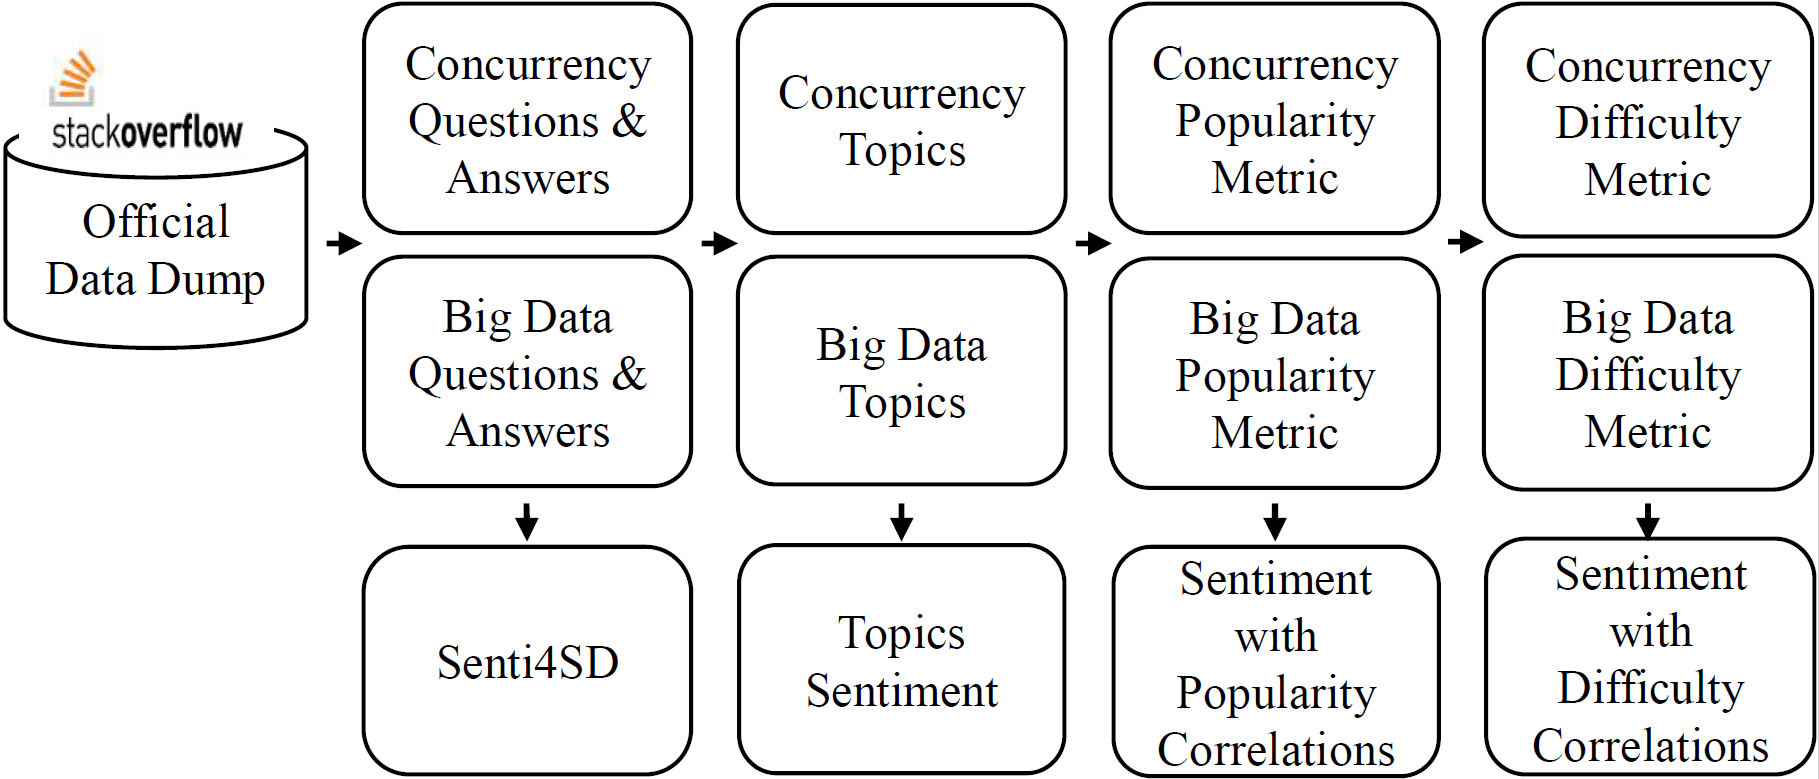
\includegraphics{Images/methodology}
\caption{Methodology}
\label{last}
\end{figure}
\def\L{\textless}
\def\G{\textgreater}
\chapter{METHODOLOGY}

In this chapter, we examine the methods used in our analysis in detail to answer the research questions \emph{\textbf{R1}} to \emph{\textbf{R4}}. We begin with the background of the Stackoverflow questions and answers. Next, our methodology to perform sentiment analysis. Finally, we discuss the methods to find whether correlations exist within the datasets.

\section{Stackoverflow Questions and Answers}
It is essential to understand the structure of Stackoverflow questions and answers and their usage in our analysis. When a registered Stackoverflow participant posts a question related to software topics, the post generates question metadata. Similarly, when a participant answers the posted question, it generates answer metadata. When the participant requesting the question receives a relevant answer, the most relevant answer becomes an accepted answer. The Stackoverflow participant and platform are the two sources that generate the question metadata. The participant generates the question title, descriptive question body, relevant tags, and accepted answer. While the Stackoverflow platform generates the unique identifier, date and time of the post, the number of favorites, score, and the number of views to the question. 

Similarly, the answer metadata has two sources, where the participant generates the answer body, and the platform generates the answer identifier and date. When participants post duplicate questions, the Stackoverflow platform often merges the two questions into one. If a participant considers and marks an answer as a relevant solution for this problem, then the Stackoverflow platform considers that answer as an accepted answer. For an example question and answer metadata, refer to the Table \ref{questions} and the Table \ref{answers} and note the metadata updates with time.

\begin{table}[t!hb]
\caption{Stackoverflow Sample Question}
\label{questions}
% this question has neutral sentiment: positive
\centering
\begin{tabular}{p{1.7in}p{1.5in}p{2.5in}} \hline
\textbf{Question Metadata} & \textbf{Description} & \textbf{Example}\\ \hline
question id & unique identifier & 47613802\\ 
\\
title & title given by user & how to create threads dynamically? \\
\\
body & question content & I want to create certain number of threads in my program where the number of threads to be created is provided by the user at run-time\\
\\
date & time and date of post & 2017-12-02 23:44:13.160\\ 
\\
tags & Stackoverflow tags & multithreading, java, dynamic\\
\\
favorites & count of user likes & 79\\ 
\\
score & like and dislike score & 150\\
\\
views & total views & 454\\
\\
accepted answer & user accepted answer & 47613819 \\ \hline
\end{tabular}
\end{table}


\begin{table}[b!ht]
\caption{Stackoverflow Sample Answer}
\label{answers}
\centering
\begin{tabular}{p{1.7in}p{1.5in}p{2.5in}} \hline
\textbf{Answer Metadata} & \textbf{Description} & \textbf{Example}\\\hline
answer id & a unique identifier & 47613819 \\ 
\\
date & time and date of post & 2017-12-02 23:47:28.157 \\
\\
body & an answer to question & there are a number of ways to do this. A for loop is the easiest your runnable couple be something like this\\ \hline
\end{tabular}
\end{table}


\section{Concurrency and Big Data Datasets}

To perform our sentiment analysis study, we begin by examining the data for concur- rency \cite{ahmed2018concurrency} and big data \cite{bagherzadeh2019going} by using the two datasets from the previous publications. These two papers analyze the Stackoverflow question and answer posts from the Stackoverflow official data dump, which is publicly available at \cite{stackoverflow2019}. In this section, we discuss the contents of the two datasets, as shown in Figure \ref{last}; these are the questions and answers, the topics, and the measures for popularity and difficulty metrics.

\subsection{Concurrency and Big Data Questions and Answers}
\label{dataset}
For concurrency dataset, we utilized Ahmed and Bagherzadeh's work \cite{ahmed2018concurrency}, which analyzes the Stackoverflow data over 9 years from August 2008 until December 2017. This dataset includes 38,485,046 questions and answers posted by 3,589,412 software developer participants of the Stackoverflow platform. Among these posts, 14,995,834 (39\%) are questions and 23,489,212 (61\%) are answers. From 38,485,046 questions and answers, the study concluded by identifying 245,576 (64\%) of questions and answers belonging to the topic of concurrency. In those concurrency posts of the total of 245,576 questions and answers, 156,812 (64\%) belong to question posts and 88,764 (36\%) belonging to answer posts.

To study big data developers, we utilized the data from Bagherzadeh and Khatchad- ourian \cite{bagherzadeh2019going} work, which categorizes Stackoverflow questions and answers as big data topics. The input dataset for the study includes 42,850,541 Stackoverflow questions and answers posted by 4,142,516 software developers over a 10-year duration from August 2008 to December 2018. The study identifying 157,525 questions and answers belonging to big data topics of those, 112,948 (72\%) are questions, and 44,577 (28\%) are answers. Our study aggregates both papers, and our dataset input has 403,413 questions and answers containing 269,818 (67\%) questions and 133,595 (33\%) answers. To see the statistics of our dataset, refer to Table \ref{tabStat}. We perform sentiment analysis on 403,413 questions and answers to answer our research questions.

\subsection{Concurrency and Big Data Topics} 
\label{topicssec}
To study the sentiment of concurrency and big data topics, we utilize the topic categorization conducted by the papers \cite{ahmed2018concurrency, bagherzadeh2019going}. These two works categorize the questions and answers using Latent Dirichlet Allocation (LDA) \cite{blei2003latent} and an open card sort. Topic modeling using LDA means assigning related topic names over a normal distribution based on keywords existing in the question and answer. And, an open card sort means that topic names are not predefined but assigned in the topic labeling process. The topic labeling process the studies \cite{ahmed2018concurrency, bagherzadeh2019going} follow, is that they manually sample through 15 random posts from individual topics. By iteratively refining associated topics, 27 topics names were manually assigned to 245,576 concurrency questions and answers. To see the concurrency topic names and their descriptions, refer to Table \ref{tab:CT}. For 157,525 big data questions and answers, the study \cite{bagherzadeh2019going} assigns them to 28 big data topics. For detailed big data topic names and descriptions, refer to Table \ref{tab:BT}. We perform sentiment analysis to assess sentiments for each topic in concurrency and big data datasets.

\begin{table}[h!bt]
\caption{Statistics of Concurrency and Big Data Dataset}
\label{tabStat}
\centering 
\begin{tabular}{p{.9in}p{1.4in}p{1.4in}p{1.4in}} \hline
\textbf{Dataset} & \textbf{No. of Q\&As} & \textbf{No. of Questions} & \textbf{No. of Answers}\\  \hline
concurrency & 245,576 & 156,812 (64\%) & 88,764 (36\%) \\
\\
big data & 157,525 & 112,948 (72\%) & 44,577 (28\%) \\\hline
\textbf{Total} & \textbf{403,413} & \textbf{269,818 (67\%)} & \textbf{133,595 (33\%)} \\ \hline
\end{tabular}
\end{table}

\begin{table}[tbp]
\caption{Concurrency Topics From the Previous Work \cite{ahmed2018concurrency}}
\centering
\label{tab:CT}
\begin{tabular}{p{.15in}p{2.25in}p{3.1in}}\hline
%\textbf{No.}&\textbf{Topic}&\textbf{Topic Description for Q \& A's }\\ \hline
\textbf{No.}&\textbf{Topic}&\textbf{Q \& As Topic Words}\\ \hline
1&basic concepts & 
code understand read find edit make\\

2&task parallelism & 
task schedul async asynchron parallel\\

3&producer-consumer concurrency & 
queue consum produc process buffer block\\

4&parallel computing & 
parallel node loop comput openmp mpi\\

5&process life cycle management& 
process child parent termin fork kill start\\

6&python multiprocessing& 
python script run multiprocess parallel php\\

7&thread life cycle management& 
thread execut background separ join finish\\

8&thread sharing& 
variabl pass call pointer pthread global\\

9&thread scheduling& 
loop time wait stop run start sleep set check\\

10&thread pool & 
pool job process task limit threadpool\\

11&concurrent collections& 
list arrai map element collect iter kei add\\

12&thread safety& 
thread java safe multipl multi multithread\\

13&locking& 
lock mutex wait condit semaphor acquir\\

14&memory consistency& 
read write variabl atom cach share synchron\\

15&entity management& 
concurr session spring entiti transact actor\\

16&database management systems& 
databas tabl queri row record lock insert sql\\

17&file management& 
file read write log line open stream directori\\

18&object-oriented concurrency& 
object class method creat static access\\

19&web concurrency& 
servic web server applic user app net http\\

20&event-based concurrency& 
event signal handler timer callback call slot\\

21&mobile concurrency& 
android app view updat frame asynctask\\

22&client-server concurrency& 
connect send socket receiv port read\\

23&data scraping& 
data time load download problem\\

24&runtime speedup& 
cpu core time performance\\

25&unexpected output& 
code work run output problem print line\\

26&irreproducible behavior& 
error run problem applic compil crash\\

27&GUI& 
updating gui windows applications\\ \hline
\end{tabular}
\end{table}

\begin{table}[tbp]
\caption{Big Data Topics From the Previous Work \cite{bagherzadeh2019going}}
\centering
\label{tab:BT}
\begin{tabular}{p{.15in}p{2.25in}p{3.1in}}\hline
\textbf{No.}&\textbf{Topic}&\textbf{Q \& As Topic Words}\\ \hline
1&memory management & 
memori executor task job spark run core\\ 

2&PIG& 
pig scripts oozi job workflow action run error\\ 

3&connection& 
connect hadoop server instal cloudera\\ 

4&dataset load\&store & 
file data spark read json csv parquet load\\ 

5&data organization& 
partit join data number case oper kei set\\ 

6&scala spark& 
scala spark org apach java sql appli anonfun\\ 

7&pyspark& 
python pyspark spark zeppelin error run\\ 

8&dataframe& 
column datafram row spark pyspark data\\ 

9&file distribution& 
node hadoop cluster namenod hdf datanod\\

10&general programming& 
class function method object call code type\\ 

11&debugging& 
error code run work problem issu except fail\\ 

12&hbase& 
hbase tabl row region zookeep client scan\\ 

13&job management& 
spark run cluster job applic submit yarn\\ 

14&file format& 
file line read input split text block size data\\

15&file management& 
file hdf directori path hadoop folder local\\ 

16&string& 
string type field arrai null column valu\\ 

17&database import\&export& 
sqoop cassandra jdbc mysql databas connector\\ 

18&stream processing& 
stream spark kafka data messag batch process\\ 

19&basic concepts& 
data hadoop process system databas solut\\ 

20&date\&time& 
date time timestamp data month event record\\ 

21&logging& 
info flume log java org channel apach sink\\ 

22&performance& 
data perform memori process size run million\\ 

23&text search& 
document mongodb queri collect elastic search\\ 

24&dependency management& 
jar hadoop version spark java error run depend\\ 

25&debugging& 
java org apach hadoop lang run mapr util\\ 

26&machine learning& 
model spark vector mahout train featur data\\ 

27&hive analysis& 
hive tabl queri creat data sql select insert\\ 

28&mapreduce& 
kei group count reduc hadoop map reduc\\ 

29&RDD& 
rdd spark transform code function scala map\\ \hline
\end{tabular}
\end{table}

\clearpage
\subsection{Concurrency and Big Data Popularity and Difficulty}
We utilized popularity and difficulty metrics for the concurrency and big data topics from \cite{ahmed2018concurrency, bagherzadeh2019going} to determine the correlation between sentiment with popularity and sentiment with difficulty. The authors evaluated popularity and difficulty metrics using questions and answers metadata of the Stackoverflow, given in Table \ref{questions} and the Table \ref{answers}. The popularity metric was calculated by 3 well-known measures, which are the average views, average favorites, and average scores. Likewise, they evaluated the difficulty metric using 2 well-known measures, which are the percentage of questions without accepted answers and the hours to receive an accepted answer.

To be more specific, the definitions of the popularity metrics are as follows; they defined average views measure \cite{bajaj2014mining, nadi2016jumping, rosen2016mobile, yang2016security} as the average number of visits to the posted question to the number of questions in a topic. They considered the average views measure because Stackoverflow allows both registered and unregistered users to visit questions. We consider average views because the number of views to the Stackoverflow platform by the unregistered users is higher in number compared to registered users \cite{mamykina2011design}. Secondly, as defined in \cite{bajaj2014mining, nadi2016jumping, pinto2015study, yang2016security}, the average favorites measure uses the question metadata’s favorites counter by taking the average of it within a topic. To be more specific, the average favorites is the total number of registered users who mark the question as to their favorites. Finally, as defined in \cite{bajaj2014mining, nadi2016jumping, pinto2015study, yang2016security}, the average scores measure is calculating the average of the question metadata’s scores counter within a topic. To be more specific, the average scores is the total number of registered users who like or dislike the question. For more details about popularity metrics, refer to Table \ref{PM}.

\begin{table}[h!tb]
\caption{Popularity and Difficulty Metrics}
\label{PM}
\centering
\begin{tabular}{p{0.70in}p{1.20in}p{3.60in}} \hline
\textbf{Metrics} & \textbf{Measures} & \textbf{Description}\\ \hline
popularity & average views & an average number of views for all the questions in a topic the questions in a topic \\
\\
& average favorites & total average of users marking the question as their as their favorite in a topic \\
\\
& average scores & average of raw score for all the questions within a topic \\
\\
difficulty & \%w/o acc. answer & percentage of questions without accepted answers \\
\\
& hrs to acc. answer & average median time needed for questions of a topic to receive accepted answers\\ \hline
\end{tabular}
\end{table}

On the other hand, the difficulty metric defined 2 measures that are as follows. The first measure the percentage of questions that do not have accepted answers within a topic \cite{rosen2016mobile, treude2011programmers,yang2016security}. The second measure checks the average time that is taken for a question in a topic to receive an accepted answer \cite{rosen2016mobile, yang2016security}. More straightforward questions tend to receive solutions faster compared to harder questions. Measures of the difficulty metric are in Table \ref{PM}.

The authors in \cite{ahmed2018concurrency, bagherzadeh2019going} calculated popularity and difficulty metrics for concurrency and big data topics using the five measures defined as above. Note, the values calculated for the measures dependent on questions and answers metadata and the time the information is gathered. The values for the popularity and difficulty measures for the concurrency topics are in the Table \ref{CP}. Likewise, the values for these two measures for the big data topics are in Table \ref{BP}.

\begin{table}[tbp]
\caption{Popularity and Difficulty Metrics for the Concurrency Topics From the Previous Work \cite{ahmed2018concurrency}}
\label{CP}
%\begin{tabular}{p{1.5in}p{.6in}p{.6in}p{.6in}p{.7in}p{.6in}} \hline
\begin{tabular}{p{1.7in}p{.5in}p{.6in}p{.4in}p{.9in}p{.9in}} \\ \hline
\textbf{Topic} & \textbf{Popularity} & & & \textbf{Difficulty} \\\hline
& \textbf{Avg. views} & \textbf{Avg. favorites} & \textbf{Avg. scores} & \textbf{\%w/o acc. answer} & \textbf{Hrs to acc. answer}\\ \hline
thread safety & 2848 & 1.5 & 4.6 & 39.6 & 0. 3\\ 
basic concepts & 2222 & 1.6 & 4.3 & 37.0 & 0.7 \\ 
task parallelism & 2216 & 1.3 & 4.0 & 35.3 & 0.4 \\ 
locking & 2152 & 1.3 & 3.5 & 40.1 & 0.3\\ 
thread life cycle management & 2130 & 0.7 & 2.4 & 40.4 & 0.3\\ 
thread scheduling & 2032 & 0.7 & 2.2 & 40.8 & 0.4\\ 
process life cycle management & 2004 & 1.0 & 2.6 & 44.9 & 0.6\\ 
thread pool & 1841 & 0.9 & 2.7 & 47.0 & 0.7\\ 
object-oriented concurrency & 1773 & 0.8 & 2.6 & 35.2 & 0.3\\ 
database management systems & 1727 & 0.6 & 1.8 & 51.2 & 1.0\\ 
thread sharing & 1671 & 0.6 & 2.0 & 35.6 & 0.3\\ 
GUI & 1664 & 0.5 & 1.6 & 41.1 & 0.4\\ 
irreproducible behavior & 1647 & 0.6 & 2.3 & 51.1 & 2.1\\ 
event-based concurrency & 1636 & 0.7 & 2.3 & 39.7 & 0.6 \\ 
python multiprocessing & 1587 & 0.9 & 2.5 & 50.3 & 0.9 \\ 
entity management & 1583 & 0.8 & 2.3 & 48.0 & 1.8\\ 
memory consistency & 1531 & 1.7 & 4.8 & 33.2 & 0.4\\ 
file management & 1458 & 0.6 & 1.9 & 48.8 & 0.6\\ 
producer-consumer concurrency & 1311 & 0.8 & 2.2 & 43.3 & 0.7\\ 
unexpected output & 1304 & 0.5 & 1.6 & 41.8 & 0.7\\ 
mobile concurrency & 1292 & 0.5 & 1.3 & 50.4 & 0.8\\ 
runtime speedup & 1276 & 0.9 & 2.7 & 48.0 & 0.7\\ 
web concurrency & 1252 & 0.8 & 1.9 & 50.7 & 0.9 \\ 
concurrent collections & 1155 & 0.5 & 2.0 & 38.6 & 0.4 \\ 
client-server concurrency & 1083 & 0.4 & 1.1 & 50.4 & 0.9\\ 
data scraping & 1003 & 0.6 & 1.4 & 48.9 & 1.0 \\ 
parallel computing & 899 & 0.6 & 1.9 & 50.1 & 2.1\\ \hline
\textbf{Average} & \textbf{1640.6} & \textbf{0.8} & \textbf{2.4} & \textbf{43.7} & \textbf{0.7}\\ \hline
\end{tabular}
\end{table}

\begin{table}[tbp]
\caption{Popularity and Difficulty Metrics for the Big Data Topics From the Previous Work \cite{bagherzadeh2019going}}
\label{BP}
\centering
\begin{tabular}{p{1.4in}p{.5in}p{.6in}p{.4in}p{.9in}p{.9in}} \hline
% \begin{tabular}{p{1.8in}p{.4in}p{.6in}p{.4in}p{.9in}p{.9in}} \hline
\textbf{Topic} & \textbf{Popularity} & & & \textbf{Difficulty} \\ \hline
& \textbf{Avg. views} & \textbf{Avg. favorites} & \textbf{Avg. scores} & \textbf{\%w/o acc. answer} & \textbf{Hrs to acc. answer}\\ \hline
file management & 2141.6 & 0.5 & 1.4 & 62.3 & 3.7 \\
file distribution & 1861.6 & 0.5 & 1.3 & 63.1 & 6.7 \\
hive & 1811.6 & 0.3 & 1.0 & 66.0 & 3.6\\
dependency management & 1774.7 & 0.4 & 1.4 & 64.2 & 4.7\\
dataframe & 1731.4 & 0.5 & 1.3 & 46.3 & 1.2 \\
string & 1600.8 & 0.3 & 1.0 & 51.9 & 1.3\\
RDD & 1543.8 & 0.5 & 1.6 & 49.4 & 1.1\\
hbase & 1464.9 & 0.4 & 1.3 & 63.4 & 17.2 \\
dataset load\&store & 1410.7 & 0.4 & 1.2 & 63.5 & 2.9\\
data organization & 1369.3 & 0.8 & 2.0 & 58.5 & 3.2\\
file format & 1315.1 & 0.5 & 1.2 & 61.9 & 4.0\\
connection management & 1301.7 & 0.3 & 1.0 & 68.7 & 17.0\\
mapreduce model & 1294.2 & 0.5 & 1.2 & 51.6 & 0.2\\
debugging & 1278.3 & 0.3 & 1.2 & 64.3 & 2.4\\
basic concepts & 1248.7 & 0.9 & 1.8 & 59.8 & 5.5\\
pyspark & 1152.5 & 0.4 & 1.3 & 68.1 & 7.6 \\
memory management & 1141.1 & 0.6 & 1.7 & 69.0 & 7.7 \\
job management & 1131.2 & 0.4 & 1.5 & 65.7 & 9.2 \\
general programming & 1130.9 & 0.5 & 1.6 & 53.8 & 1.8\\
PIG & 1079.8 & 0.2 & 0.8 & 63.0 & 10.1 \\
date\&time & 1068.1 & 0.3 & 0.7 & 55.8 & 2.1 \\
text search & 1053.8 & 0.5 & 1.3 & 57.5 & 5.2\\
scala spark & 1050.0 & 0.3 & 1.0 & 64.8 & 2.6\\
database import\&export & 1048.7 & 0.3 & 0.8 & 69.8 & 7.9 \\
performance & 840.3 & 0.5 & 1.4 & 64.0 & 3.8\\
logging & 820.7 & 0.3 & 0.8 & 66.9 & 22.5 \\
machine learning & 763.9 & 0.5 & 1.3 & 61.6 & 4.6\\
stream processing & 715.0 & 0.4 & 1.2 & 71.3 & 7.4\\ \hline
\textbf{Average} & \textbf{1290.8} & \textbf{0.4} & \textbf{1.2} & \textbf{61.6} & \textbf{5.9} \\ \hline
\end{tabular}
\end{table}

\section{Sentiment Analysis}

To perform our sentiment analysis, we followed the following steps: For Step 1, we removed noise by preprocessing the Stackoverflow question and answers. In Step 2, we analyzed the sentiment of Stackoverflow questions and answers by using the tool Senti4SD for concurrency and big data datasets. In Step 3, we measured the sentiment for topics in the concurrency and the big data topics, which are in the Tables \ref{tab:CT} and the Table \ref{tab:BT}, respectively. In the final step, we calculated correlations between sentiment with popularity and sentiment with difficulty using Kendall Tau bivariant correlation. 

\subsection{Preprocessing}
Determining the sentiment of text with noise could lead to incorrect results. So, the text should be free of hidden metadata to perform the sentiment analysis. Consequently, we preprocessed the body of the questions and the body of the answer to reduce noise. A more thorough explanation for the preprocessing is getting a plain text, which we define as a piece of text containing alphanumeric characters.

We start by removing the code snippets that contain code using natural language processing. That is, we removed the tags {\L/code\G} and {\L/code\G} from the questions and answers metadata. Then, we remove all remaining HTML tags such as paragraph tags {\L/p\G} and {\L/p\G}, URL tags {\L/a\G} and {\L/a\G} and nbsp; extra spaces tag. 

\begin{table}[b!ht]
\caption{Preprocessing Example}
\label{tab:example}
\centering
% {|lll|}SSS
\begin{tabular} {p{3in}p{2.5in}}\hline
\textbf{Input Text} & \textbf{Processed Text} \\ \hline

body: \&lt;p\&gt; i use retrofit to get the response correctly, then i pass the response to an object in the response body, while it fails to get the object in, ui thread there is a nullpointerexception, error i think it's the problem of the asynchronous request, how can i avoid this problem? \&lt;p\&gt;?\&lt;/p\&gt; \&\#xA;\&\#xA;\&lt;pre\&gt;\&lt;code\&gt; \emph{multiple lines of code in java} \&\#xA;\&lt;/code\&gt;\&lt;/pre\&gt;\&\#xA;
&
i use retrofit to get the response correctly then i pass the response to an object in the response body while it fails to get the object in ui thread there is a nullpointerexception error i think it's the problem of asynchronous request how can i avoid this problem \emph{(removed)} \\ \hline
\end{tabular}
\end{table}

Furthermore, we removed any remaining newlines, extra spaces, and non-alphanum- eric characters using the Java library JSoup to parse the text and convert it to a plain text.

We preprocessed 400K Stackoverflow questions and answers to plain text that belong to both concurrency and big data datasets. For instance, a question's metadata before and after preprocessing can be seen in Table \ref{tab:example}. Here, the text in the left column represents the text before preprocessing, and the text in the right column gives the processed version of the same text.

\subsection{Senti4SD}

We utilize the tool Senti4SD to assess the sentiment, which can be either positive, negative, or neutral for the 400K Stackoverflow questions and answers belonging to both concurrency and big data datasets. For more details about the tool, Senti4SD refer \cite{calefato2018sentiment}. 

As discussed in section \ref{dataset}, the 400K Stackoverflow questions and answers are an aggregate of 250K concurrency dataset and 150K big data dataset. The sentiment analysis on this dataset performed, as shown in Figure \ref{step1}. A sample of Stackoverflow question processed by the Senti4SD tool is shown in the Table \ref{SE}, where the input is a preprocessed text as seen in the left column, and the output sentiment assessment for this text is in the right column.


\begin{table}[h!tb]
\caption{A Sample Stackoverflow Question and Its Sentiment}
\label{SE}
\centering
\begin{tabular}{p{3.5in}p{2in}}\hline
\textbf{Processed Text} & \textbf{Sentiment of Text} \\\hline
{i use retrofit to get the response correctly then i pass the response to an object in the response body while it fails to get the object in ui thread there is a nullpointerexception error i think it's the problem of the asynchronous request how can i avoid this problem} & {positive} \\ \hline 
\end{tabular}
\end{table}

\begin{figure}[h!tb]
\centering 
\includegraphics{Images/Sentiment}
\caption{Sentiment Analysis Using Senti4SD}
\label{step1}
\end{figure}

\subsection{Concurrency and Big Data Topics Sentiment}
\label{topicsenti}
In the previous section, we discussed the sentiment analysis tool Senti4SD to assess the sentiment of questions and answers belonging to concurrency and big data datasets. As the goal of our thesis is to answer the research questions \emph{\textbf{R1}} to \emph{\textbf{R4}}, we do so by understanding the relationship between a software developer's sentiment concerning popular and difficult concurrency and big data topics. We calculate the topic sentiment by taking the mean of the sentiment assessments (positive, negative, neutral) for all the Stackoverflow questions and answers within a topic.

\subsection{Correlations in Concurrency and Big Data}
\label{correlations}
To find the correlations within the concurrency and big data datasets, first, we gathered the results from our previous step of finding sentiment for each topic within these datasets. Next, we used the popularity and difficulty metrics calculated by the authors in \cite{ahmed2018concurrency, bagherzadeh2019going}. In total, our research finds correlations between three measures of sentiment with three measures of popularity metric and three measures of sentiment with two measures of difficulty metric. 

We find the correlations existing within concurrency and big data datasets using a rank-based correlation. For this, we use Kendall tau bivariant correlation, which in comparison to other rank-based correlations, is less sensitive to outliers, giving us relatively many stable results. Kendal tau computes the coefficient between two non-parametric variables belonging to the same set with different ranks. To test our hypothesis of statistical dependencies, we input our numerical results to the tool IBM SPSS \cite{IBM2019}. A non-parametric test means that the distribution is without any underlying assumptions. In short, it means that the distribution has no prior knowledge about the probabilities of the variables being assessed.

By evaluating the correlations given by the tool, we answer our research questions \emph{\textbf{R1}} to \emph{\textbf{R4}}. The flow of our analysis is in Figure \ref{last}. In the next chapter, we discuss our results in depth.

\begin{figure}[h!tb]
\centering
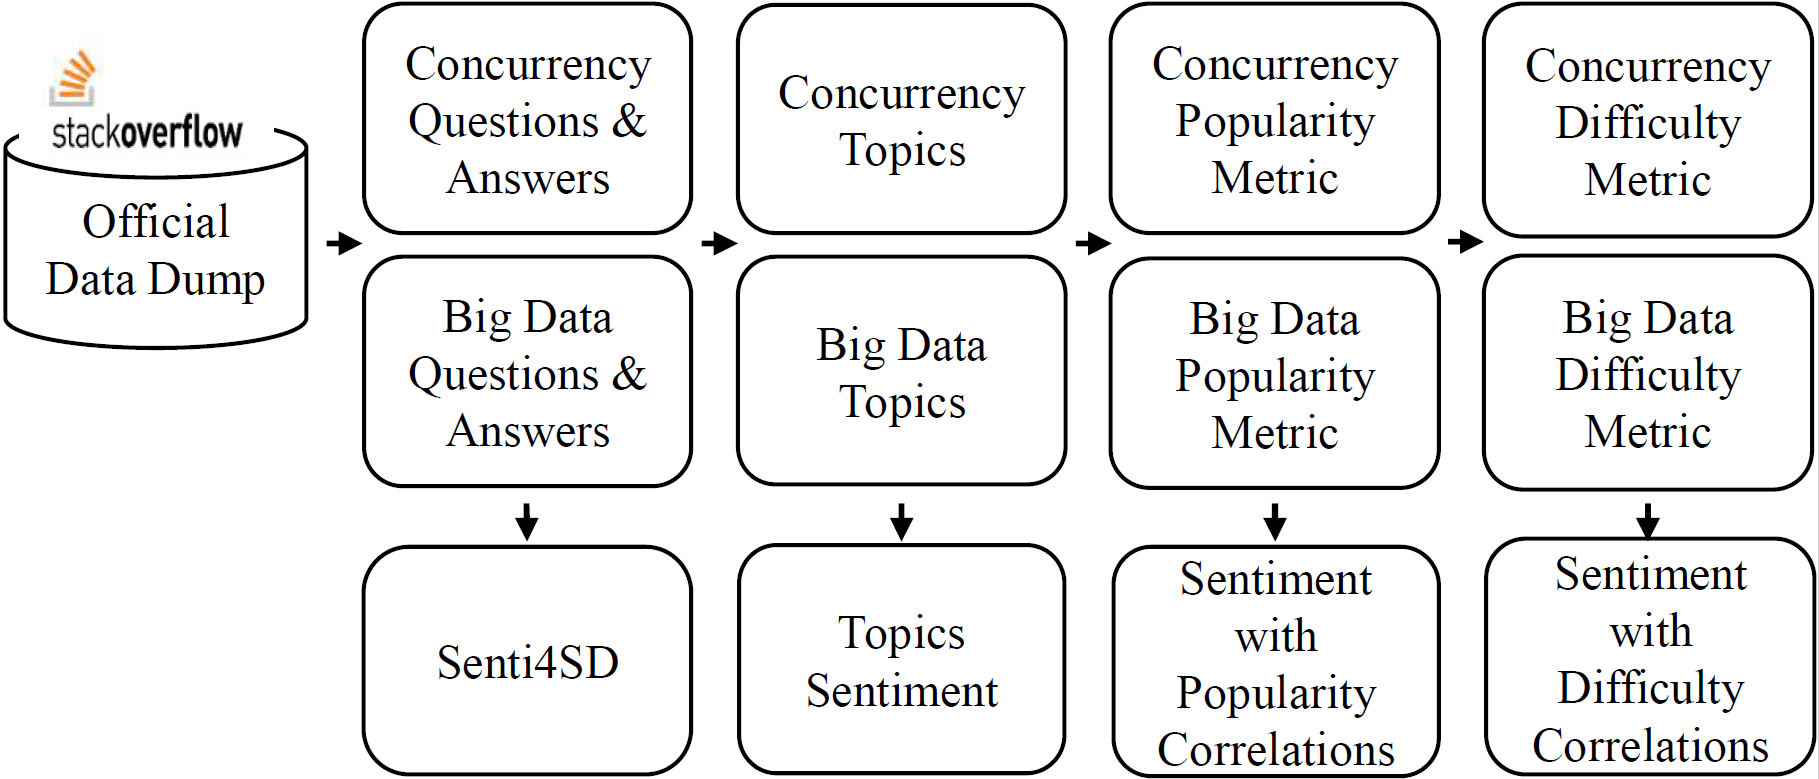
\includegraphics{Images/methodology}
\caption{Methodology}
\label{last}
\end{figure}
% Results
\chapter{RESULTS}
In this chapter, we present the discussion of our research findings for concurrency and big data datasets. First, we present the results of our sentiment analysis. Next, we analyze the correlations. Finally, we conclude this chapter by answering our research questions \emph{\textbf{R1}} to \emph{\textbf{R4}} with a detailed analysis of the results for both concurrency and big data datasets.

\section{Concurrency and Big Data Sentiment}
In this section, we present our results for concurrency and big data dataset topics sentiment. 

Initially, we calculate the sentiment percentages for each topic within the concurrency dataset, which we presented in Table \ref{tab:CT}. We compute the sentiment percentages for the concurrency topics by evaluating the sentiment for all the questions and answers and take the mean of sentiments measure (positive, negative, neutral) for a topic. 

The results for positive, negative, neutral sentiment percentages regarding the conc- urrency dataset, are shown in Table \ref{tableSentiConcurrency}. For instance, from the table,
if we pick the positive polarity, we find that the \emph{data scraping} topic has the highest rate of positive polarity. In contrast, \emph{process life cycle management} topic has the lowest positive polarity of Stackoverflow questions and answers. The 
\emph{process life cycle management} keeps the lowest sentiment percentage in negative polarity, and \emph{irreproducible behavior} topic claims the highest negative polarity. The same two topics, \emph{process life cycle management} and \emph{irreprod- ucible behavior}, switch their polarities from lowest to highest, highest to lowest respectively in neutral polarities. Overall, concurrency sentiment analysis concludes by evaluating the mean sentiment for all the topics, which are 16.1\%, 23.4\%, and 60.2\% to positive, negative, and neutral sentiment.


Similar to the calculations we did for the concurrency, we compute the big data topics sentiment percentages. The result of our calculations is in Table \ref{tab:BT}. The resulting mean of sentiment measures (positive, negative, neutral) for each topic belonging to the big data dataset is in Table \ref{tab:BT}.

In the big data topic, \emph{basic concepts} topic has the highest rate of positive polarity, and \emph{scala spark} topic has less positively polarized Stackoverflow questions and answers. These two topics switch their polarities from high to low and vice versa for negative polarity. The topic \emph{general programming} has a higher percentage of questions and answers with neutral polarity, whereas \emph{debugging} topic has the lowest. Overall big data sentiment analysis concludes by evaluating the mean sentiment for all the topics, which are 16.8\%, 36.4\%, and 46.6\% to positive, negative, and neutral sentiment, respectively. 

\section{Concurrency and Big Data Sentiment Correlations}

To understand the role of the sentiment towards software developers' productivity, we find the correlations existing between sentiment with popularity and sentiment with difficulty. To do so, we gather the sentiment for each topic within concurrency and big data datasets calculated in the previous section. Then we consider the popularity and difficulty metrics computed by the authors \cite{ahmed2018concurrency, bagherzadeh2019going}, as in Table \ref{CP} and the Table \ref{BP} for concurrency and big data, respectively. Finally, using the tool IBM SPSS, we find the correlations existing in concurrency and big data datasets to answer our research questions \emph{\textbf{R1}} to \emph{\textbf{R4}}.

\begin{table}[tbp]
\caption{Concurrency Topics Sentiment}
\label{tableSentiConcurrency}
\centering
\begin{tabular}{lccc} \hline
\textbf{Topic} & \textbf{Positive} & \textbf{Negative} & \textbf{Neutral} \\ \hline
thread safety & 20.4 & 19.3 & 60.1 \\ 
basic concepts & 19.3 & 20.9 & 59.7 \\ 
task parallelism & 13.5 & 20.0 & 66.3 \\
locking & 9.6 & 18.6 & 71.6 \\ 
thread life cycle management & 10.7 & 22.6 & 66.5 \\ 
thread scheduling & 14.3 & 28.4 & 57.1 \\ 
process life cycle management & 7.6 & 14.0 & 78.3 \\ 
thread pool & 11.6 & 16.6 & 71.7 \\
object-oriented concurrency & 16.4 & 20.1 & 63.4 \\ 
database management systems & 21.7 & 21.4 & 56.8 \\ 
thread sharing & 10.5 & 24.5 & 64.9 \\ 
GUI& 16.7 & 30.7 & 52.4 \\ 
irreproducible behavior & 16.3 & 43.0 & 40.6 \\ 
event-based concurrency & 11.7 & 20.2 & 67.9 \\ 
python multiprocessing & 17.3 & 26.9 & 55.6 \\ 
entity management & 21.5 & 20.1 & 58.2 \\ 
memory consistency & 15.0 & 16.8 & 68.1 \\ 
file management & 12.1 & 18.5 & 69.3 \\ 
producer-consumer concurrency & 14.4 & 23.1 & 62.4 \\ 
unexpected output & 18.3 & 36.9 & 44.7 \\ 
mobile concurrency & 19.4 & 31.1 & 49.4 \\ 
runtime speedup & 16.6 & 20.9 & 62.4 \\ 
web concurrency & 18.2 & 22.6 & 59.1 \\ 
concurrent collections & 20.3 & 16.8 & 62.8 \\ 
client-server concurrency & 16.9 & 30.8 & 52.1 \\ 
data scraping & 26.7 & 27.7 & 45.5 \\ 
parallel computing & 18.8 & 20.8 & 60.3 \\ \hline
\textbf{Average} & \textbf{16.1} & \textbf{23.4} & \textbf{60.2} \\ \hline
\end{tabular}
\end{table}


\begin{table}[tbp]
\caption{Big Data Topics Sentiment}
\label{tab:SentiBigdata}
\centering
\begin{tabular}{lccc} \hline
\textbf{Topic} & \textbf{Positive} & \textbf{Negative} & \textbf{Neutral} \\ \hline
file management & 11.3 & 28.9 & 59.7 \\
file distribution & 15.1 & 38.4 & 46.3 \\ 
hive & 20.6 & 36.7 & 42.6 \\
dependency management & 12.3 & 48.5 & 39.0 \\
dataframe & 20.7 & 27.9 & 51.3 \\
string & 19.6 & 23.7 & 56.5 \\
RDD& 16.2 & 30.6 & 53.1 \\
hbase & 22.4 & 29.2 & 48.2 \\
dataset load\&store & 16.9 & 35.3 & 47.7 \\
data organization & 14.2 & 27.6 & 58.0\\
file format & 15.3 & 29.3 & 55.3 \\
connection management & 15.9 & 43.8 & 40.2 \\
mapreduce model & 21.3 & 26.4 & 52.2 \\
debugging & 15.8 & 54.2 & 29.9 \\
basic concepts & 25.2 & 23.3 & 51.3 \\
pyspark & 13.1 & 51.1 & 35.7 \\
memory management & 15.2 & 38.4 & 46.3 \\
job management & 11.8 & 41.6 & 46.4 \\
general programming & 14.0 & 24.1 & 61.7 \\
PIG & 16.2 & 43.3 & 40.4 \\
date\&time & 20.8 & 29.2 & 49.8 \\
text search & 18.1 & 32.1 & 49.7 \\
scala spark & 6.4 & 54.8 & 38.6 \\
database import\&export & 18.4 & 43.5 & 37.9 \\
performance & 20.9 & 36.6 & 42.3 \\
logging & 17.1 & 40.1 & 42.6 \\
machine learning & 20.1 & 38.6 & 41.2 \\
stream processing & 15.6 & 43.0 & 41.2 \\ \hline
\textbf{Average} & \textbf{16.8} & \textbf{36.4} & \textbf{46.6}\\ \hline
\end{tabular}
\end{table}


\begin{table}[t!hb]
\caption{Correlations in Concurrency}
\label{tab:ConcPopl}
\centering
\begin{tabular}{p{0.7in}p{1.7in}p{0.7in}p{0.7in}p{0.7in}} \hline
\textbf{Metric} & \textbf{Measure} & \textbf{Positive} & \textbf{Negative} & \textbf{Neutral} \\
\hline
popularity & average views & -/.01849 & -/.14996 & +/.07294 \\
\\
& average favorites & -/.19815 & \hl{-/.00154} & +/.00889 \\ 
\\
& average scores & +/.07911 & \hl{-/.00127} & \hl{+/.00320} \\
\\
difficulty & \% w/o acc. answer & +/.08344 & +/.02289 & -/.00758 \\
\\
& hrs. to acc. answer & +/.00731 & +/.08687 & \hl{-/.00565} \\ \hline
\end{tabular}
\end{table}

We discussed the IBM SPSS tool to find the correlations. Using this methodology, the results of our correlations for the concurrency dataset are shown in the Table \ref{tab:ConcPopl}. In our computations, we found a negative correlation exists between the popularity metric's average favorites measure and negative sentiment with a correlation significance at 0.001. This means that, if the questions and answers within a concurrency topic are tilted towards the negative end of the emotions scale, then the users marking these questions and answers as their favorite are fewer. Also, there exists a positive correlation between the popularity metric's average scores measure and neutral sentiment with a significance at 0.003, which means that the neutrally toned questions and answers receive higher scores by the users.

\begin{table}[t!hb]
\caption{Correlations in Big Data}
\label{tab:PoplCorr}
\centering

\begin{tabular}{p{0.7in}p{1.7in}p{0.7in}p{0.7in}p{0.7in}} \hline
\textbf{Metric} & \textbf{Measure} & \textbf{Positive} & \textbf{Negative} & \textbf{Neutral} \\
\hline
popularity & average views & -/.60734 & -/.13308 &.04802 \\
\\
& average favorites & +/.96703 & \hl{-.00292} & \hl{+/.00406} \\ 
\\
& average scores & -/.22997 & -/.07308 & .04983 \\
\\
difficulty & \% w/o acc. answer & -/.13308 & \hl{+/.00006} & \hl{-/.00009} \\
\\
& hrs. to acc. answer & -/.63265 & .00908 & -/.01964 \\ \hline
\end{tabular}
\end{table}

Using the same approach in handling the big data dataset, the results of the correlati- ons we computed were presented in Table \ref{tab:PoplCorr}. Our popularity results indicate that there is a negative and positive correlation between negative and neutral sentiment, respectively, with respect to the average favorites. On the other hand, our difficulty metric results point that there exists a positive and negative correlation between negative and neutral sentiment, respectively, with the percentage of questions with an accepted answer measure. At this point in our analysis, we have the results to answer our research questions.

\section{Discussion}
\label{finalSectionResults}

We answer the research questions \emph{\textbf{R1}} to \emph{\textbf{R4}} introduced at the beginning of this thesis, using the correlations in concurrency and big data datasets, which can be found in the Tables \ref{tab:ConcPopl} and the Table \ref{tab:PoplCorr}. The summary of these correlations are in the Tables \ref{finalCDCorr} and in the Table \ref{finalBDCorr}.

\begin{table}[h!tb]
\caption{Summary of the Concurrency Sentiment Correlations}
\label{finalCDCorr}
\centering
\begin{tabular}{llll} \hline
\textbf{Sentiment} & \textbf{Metric} & \textbf{Direction}&\textbf{Measure}\\ \hline
positive & popularity & & no correlation \\
\\
& difficulty & & no correlation\\
\\
negative & popularity & negative & average favorites\\
\\
& & negative & average scores\\ 
\\
& difficulty & & no correlation \\
\\
neutral & popularity & positive & average scores \\
\\
& difficulty & positive & hrs. to acc. answer \\ \hline
\\
\end{tabular}
\end{table}

\emph{\textbf{R1}}. Is there a relation between sentiment with popularity and sentiment with difficulty in concurrency topics? The summary of the popularity and difficulty metrics and their correlations with sentiment are displayed in Table \ref{finalCDCorr}. For the negative and neutral sentiment, we observe correlations between both popularity and difficulty metrics. However, we did not find any correlations between positive sentiment with both popularity and difficulty metrics.

\emph{\textbf{R2}}. Is there a relation between sentiment with popularity and sentiment with difficulty in big data topics? The summary of the popularity and difficulty metrics and their correlations with sentiment are displayed in Table \ref{finalBDCorr}. For the negative and neutral sentiment, we observe correlations between both popularity and difficulty metrics. No correlation was found between positive sentiment with popularity and difficulty measures. Likewise, during our concurrency dataset analysis, we did not find correlations between positive sentiment with popularity and difficulty.

\begin{table}[b!ht]
\caption{Summary of the Big Data Correlations}
\label{finalBDCorr}
\centering
\begin{tabular}{llll} \hline
\textbf{Sentiment} & \textbf{Metric} & \textbf{Direction}&\textbf{Measure}\\ \hline
positive & popularity & & no correlation \\
\\
& difficulty & & no correlation\\
\\
negative & popularity & negative & average favorites\\
\\
& difficulty & positive & \% w/o acc. answer\\
\\
neutral & popularity & positive & average favorites \\
\\
& difficulty & positive & \% w/o acc. answer \\ \hline
\end{tabular}
\end{table}

\emph{\textbf{R3}}. What sentiment do concurrency and big data developers express towards a common topic? The concurrency and big data sentiment values are displayed in the Table \ref{tab:ConcPopl} and Table \ref{tab:PoplCorr} respectively. The \emph{basic concepts} is a common topic in both concurrency and big data topics. The questions and answers discussed in this topic are generic to the concurrency and big data topics. \emph{Basic concepts} topic has a common property, which is that the questions and answers within these topics are more neutrally toned in both concurrency and big data datasets.

\emph{\textbf{R4}}. What commonality do the correlations hold toward concurrency and big data?
Referring to the Tables \ref{finalCDCorr} and \ref{finalBDCorr}, the commonly maintained property that our computations lead towards a negative sentiment which is inversely correlated with the average favorites measure in popularity metric.
%RelatedWorks
\chapter{IMPLICATIONS}
Studying the sentiment correlations in concurrency and big data datasets, we investi- gate the impact of our findings on different communities. The following are the
implications we deduced using the research questions \emph{\textbf{R1}} to \emph{\textbf{R4}}, regarding specific communities: software practitioners, researchers, and educators. We abbreviated the implications for practitioner's, researcher's and educator's as PI, RI, and EI respectively.

%which we answered in the section \ref{finalSectionResults}.

%Considering the significance of the correlations investigated in this study, we draw the resulting implications and group together according to the needs of researchers and software developers.

%% Significance of Our Findings to Software Development Process
\section {Practitioners}
\emph{\textbf{PI.1}} By referring to the sentiment correlations in the Table \ref{finalCDCorr} and Table \ref{finalBDCorr} consider- ing our research findings for question \emph{\textbf{R4}}. We observed that concurrency and big data developers are sensitive towards negative and neutral sentiment compared to the positive sentiment.

Using the directions observed for negative sentiment with popularity metric, we deduce that concurrency developers' average favorites and average scores measure decreases when they detect more negative sentiment in the Stackoverflow questions and answers. Similarly, big data developers' average favorites measure decreases with the negative sentim- ent in the Stackoverflow questions and answers. Again, using the directions for neutral sentiment with popularity metric, we deduce that concurrency developers' average scores measure rises when a neutral sentiment is detected in the Stackoverflow questions and answers. Likewise, for the big data developers, average favorites measure increases with a neutral sentiment. The difficulty metrics sentiment correlations show that the concurrency developers take longer to receive an accepted answer when they detect neutral sentiment. On the other hand, big data developers will have fewer Stackoverflow questions with accepted answers when they detect both negative and neutral sentiment.

\emph{\textbf{PI.2}} Our findings for research answers to \emph{\textbf{R1}} and \emph{\textbf{R2}} implies that the concurrency and the big data developers receive fewer average favorites measure when Stackoverflow questions and answers have a negative sentiment.

\emph{\textbf{PI.3}} We observed from research answer \emph{\textbf{R3}} that concurrency and big data developers commonly express neutral sentiment towards basic concepts topic.

\section {Researchers}
\emph{\textbf{RI.1}} Our research findings imply correlations between negative and neutral sentiment with popularity and difficulty metrics, refer to Table \ref{finalCDCorr} and Table \ref{finalBDCorr}. However, our research did not find a correlation between positive sentiment with popularity and difficulty with both concurrency and big data topics. Researchers can further explore the sentiment and its effects on various other metrics, not limited to popularity and difficulty. This aggregated research data to understand the human emotions coefficient can further help evolving technology that primarily depends on people.

\section {Educators}
\emph{\textbf{EI.1}} Educators in their practice can refer to the utilization of the Stackoverflow platform while solving popular and difficult topics, especially with concurrency and big data topics. Considering our findings for research question \emph{\textbf{R1}} and the sentiment correlations in the Table \ref{finalCDCorr}, educators, can help concurrency developers recognize the role of negative and neutral sentiment with average favorites, average scores and hours to accepted answer measures. Similarly, our findings for research question \emph{\textbf{R2}} and the sentiment correlations in Table \ref{finalBDCorr}, educators can assist big data developers in understanding the role of negative and neutral sentiment to receive average favorites and percentage of questions with accepted answer measures.
%RelatedWorks
\chapter{RELATED WORK}

In this section, we discuss the works that are related to our current thesis, which perform sentiment analysis.

%% 1 Guzman et al. [7]: Sentiment analysis of commit comments in GitHub: An empirical study

Guzman et al. \cite{guzman2014sentiment} focuses on the human factor by analyzing the sentiment of 60,425 commit logs. These commit logs belong to 90 of the top starred software projects on Github. For these 90 projects, they studied the relationship between sentiment with three areas, which are programming languages, team distribution, and project approvals. Their research findings conclude that commit logs for Java projects tend to be more negative, projects with more distributed teams tend to have more positive commit logs, and commit comments on Mondays are more negatively toned.

%% 2 Sinha et al. [15] : Analyzing developer sentiment in the commit log 

Sinha et al. \cite{sinha2016analyzing} expanded the data to analyze the sentiment of 2M non-empty commit logs from 28K projects using BOA \cite{dyer2013boa} tool. Their research concludes that the majority of the commit logs on GitHub projects are neutral. An interesting observation is, the projects commit logs that comprise 10\% more negative emotion in comparison with positive sentiment. For some popular projects, Wednesday and Thursday commit logs are most negatively toned. Finally, a strong positive correlation exists with the sentiment in the commit logs, and the number of files changed in the commits.

%% 3 Ortu et al. [12] : Are bullies more productive?: The empirical study of affectiveness vs. issue fixing time

In the previous research, Ortu et al. \cite{ortu2015bullies} took a different approach to perform sentiment analysis. Their study focused on human "affectiveness" and developers' producti- vity in the Agile environment. For their analysis, they performed an empirical analysis on more than 560K comments from 14 Apache projects using the Jira issue tracking system. For the "affectiveness" metric, they concentrated on emotion, sentiment, and politeness. The research conveyed that emotions reflect on software developers' problem-solving prod- uctivity. By which, developers who post joyful comments take a shorter time to fix a problem compared to the developers with gloomy comments take longer to fix a similar problem. Additionally, they analyze politeness and its complex role in the developer's productivity. 

%% 4 Souza and Silva [16] : Sentiment analysis of Travis CI builds

Souza and Silva \cite{souza2017sentiment} analyzed the sentiment of the commit logs belonging to the Travis CI continuous integration server. Their dataset includes 1,262 Github projects. Concluding that the build process can both be "affects" and "affected" by negative sentiment, and developers writing continuous integration servers are more positive while writing com- mit messages. 

%% 5 Garcia et al. [4] : The role of emotions in contributors activity: A case study on the GENTOO community

Garcia et al. \cite{garcia2013role}, performed sentiment analysis on the open-source project GENTOO using the bug tracking platform BUGZILLA, to study the relation between emotions and activity of contributors. The study finds that whenever strong positive emotions or negative emotions or when an unexpected emotional deviation occurs, contributors are likely to abandon the project.

%% 6 Bazelli et al [2] : On the personality traits of StackOverflow users

Bazelli et al. \cite{bazelli2013personality}, this study explores the personality traits of the Stackoverflow users by studying the relations between the sentiment of the developer's answers and their reputation. This study finds that the top-rated users express strong positive emotions in their answers compared to medium and low ranked users and that users with a higher number of favorites posts express more positive emotion than users with a lower number of favorite posts.

%% 7 Muriga et al. [10] : Do developers feel emotions? an exploratory analysis of emotions in software artifacts
Muriga et al. \cite{murgia2014developers}, studied if issue reports carry any emotional information. Their dataset uses 117 open source projects belonging to Apache software. This study confirms that issue reports reportedly have emotions that can affect design choices, maintenance activity, and colleagues.

%%\section{Using Sentiment to Identify Software Properties}

%% 1 Rahman et al. [14] : Recommending insightful comments for source code using crowdsourced knowledge

Rahman et al. \cite{rahman2015recommending}, studies automated code comment generation by analyzing 292 Stackoverflow code fragments and 5K discussion comments. The study finds that with high precision and recall, insightful comments can be extracted. 80\% of auto-generated comments are accurate, precise, concise, and useful for the participants. 

%% 2 Zhang and Hou [18] : Extracting problematic API features from forum discussions

Zhang and Hou \cite{zhang2013extracting}, proposes ways to extract problematic API features using online discussion forums, and for this analysis, they use sentiment analysis to determine the polarity of posted
sentences. This study mainly focuses on the negative sentiment for their analysis. 

%% 3 Goul et al. [5] : Managing the enterprise business intelligence app store: Sentiment analysis supported requirements engineering. 

%% 4 Panichella et al. [13]: How can i improve my app? classifying user reviews for software maintenance and evolution

Similarly, Goul et al. \cite{goul2012managing}, used sentiment analysis to determine the usefulness and interaction of employees while utilizing business intelligence apps. Panichella et al. \cite{panichella2015can}, uses sentiment analysis to determine apps usability, apps that are available on Google Play, and Apple Stores by checking users' comments and categorizing the comments as software maintenance, evolution, bug tracking and more.

The primary resource that we use in this study to perform our sentiment analysis is Ahmed and Bagherzadeh \cite{ahmed2018concurrency} for concurrency dataset. For the big data dataset, we used Bagherzadeh and Khatchadourian \cite{bagherzadeh2019going}. Specifically, it evaluates topic modeling, popularity, and difficulty metrics and their correlations. 
% Conculusion
\chapter{CONCLUSION AND FUTURE WORKS}
We have discussed our large scale sentiment analysis in this thesis. In this final chapter, we present future work and conclusion.

\section{Conclusion}

We performed sentiment analysis on a large scale dataset with 400K Stackoverflow questions and answers belonging to concurrency and big data datasets in comparison to the related work. 

We found a strong inverse correlation between the popularity metric average favorites measure with the negative sentiment in both concurrency and big data datasets. Indicating that concurrency and big data software developers expressing less negative emotions tend to gain more likes from the users. Concurrency and big data correlations demonstrate that negative and neutral sentiment has some correlations with popularity and difficulty metrics. We also found that concurrency and big data developers are not sensitive towards positive sentiment, as we did not find correlations between positive sentiment with popular- ity and difficulty. We conclude that the software developer's sentiment towards a challeng- ing task has an impact on their productivity. 

\section{Future Works}
We plan to explore the sentiment of software practitioners developing different technologies like security, programming languages, and deep learning.


% The \StartGrizzAppendices command switches the formatting for the 
% remainder of the document -- Leave this alone
\StartGrizzAppendices
\chapter*{Appendix}
\addtocontents{toc}{\protect\contentsline {chapter}{APPENDICES}{32}{}}
%\addtocontents{toc}{\vspace{\baselineskip}APPENDICES}
In this section, we provided the scattered plots for the correlations between sentiment with popularity and sentiment with difficulty, belonging to both concurrency and big data.

\begin{figure}[b!ht]
\caption{Popularity Average Views Measure With Sentiment Correlations in Concurrency}
\begin{tabular}{p{3in}p{2.5in}} \\ 
\raisebox{-.60\height}{\includegraphics[width=7.5cm, keepaspectratio]{Images/conc/1-crop}} & 
The average views measures' relation with the positive sentiment is an inverse relationship. No significant correlations found, however.\\ 
\raisebox{-.60\height}{\includegraphics[width=7.5cm, keepaspectratio]{Images/conc/2-crop}} &  
The average views measure keeps an inverse relationship with the negative sentiment. Again, no significant correlations found between them. \\
\raisebox{-.60\height}{\includegraphics[width=7.5cm, keepaspectratio]{Images/conc/3-crop}} & 
The average views measure has a direct relation with the neutral sentiment, no indication of existing correlations also.\\
\end{tabular}
\end{figure}

\begin{figure}
\caption{Popularity Average Favorites Measure With Sentiment Correlations in Concurrency}
\begin{tabular}{p{3in}p{2.5in}} \\ 
\raisebox{-.60\height}{\includegraphics[width=7.5cm, keepaspectratio]{Images/conc/4-crop}} & 
The average favorites measure has an inverse relationship with the positive sentiment. We did not find a significant correlation between them. \\ 
\raisebox{-.60\height}{\includegraphics[width=7.5cm, keepaspectratio]{Images/conc/5-crop}} & 
The average favorites measure has an inverse relationship with the negative sentiment, we found a correlation significance at 0.001.\\
\raisebox{-.60\height}{\includegraphics[width=7.5cm, keepaspectratio]{Images/conc/6-crop}} & 
The average favorites measure has a direct correlation with the neutral sentiment, and no correlations significance found. \\
\end{tabular}
\end{figure}

\begin{figure}
\caption{Popularity Average Scores Measure With Sentiment Correlations in Concurrency}
\begin{tabular}{p{3in}p{2.5in}} \\ 
\raisebox{-.60\height}{\includegraphics[width=7.5cm, keepaspectratio]{Images/conc/7-crop}} & 
The average scores measure has in an inverse relationship with the positive sentiment, no correlations found.\\ 
\raisebox{-.60\height}{\includegraphics[width=7.5cm, keepaspectratio]{Images/conc/8-crop}} & 
The average scores measure has an inverses relationship with the negative sentiment, with a correlation significance at 0.001.\\
\raisebox{-.60\height}{\includegraphics[width=7.5cm, keepaspectratio]{Images/conc/9-crop}} & 
The average score measure has a direct relation with the neutral sentiment, with a significant correlation at 0.003.\\
\end{tabular}
\end{figure}

\begin{figure}
\caption{Difficulty \%W/o Acc. Answer Measure With Sentiment Correlations in Concurrency}
\begin{tabular}{p{3in}p{2.5in}} \\ 
\raisebox{-.60\height}{\includegraphics[width=7.5cm, keepaspectratio]{Images/conc/10-crop}} & 
The \%w/o acc. answer measure with a direct relationship with the positive sentiment has no significant correlation. \\ 
\raisebox{-.60\height}{\includegraphics[width=7.5cm, keepaspectratio]{Images/conc/11-crop}} &
The  \%w/o acc. answer measure with a direct relationship with the negative sentiment has no significant correlation.\\
\raisebox{-.60\height}{\includegraphics[width=7.5cm, keepaspectratio]{Images/conc/12-crop}} & 
The \%w/o acc. answer measure with a direct relationship with the negative sentiment has no significant correlation.\\
\end{tabular}
\end{figure}

\begin{figure}
\caption{Difficulty Hrs. to Acc. Answer Measure With Sentiment Correlations in Concurrency}
\begin{tabular}{p{3in}p{2.5in}} \\ 
\raisebox{-.60\height}{\includegraphics[width=7.5cm, keepaspectratio]{Images/conc/13-crop}} & 
The hrs. to acc. answer measure with a direct relationship with the positive sentiment has no significant correlation. \\ 
\raisebox{-.60\height}{\includegraphics[width=7.5cm, keepaspectratio]{Images/conc/14-crop}} &
The hrs. to acc. answer measure with an inverse relationship with the negative sentiment has no significant correlation. \\ 
\raisebox{-.60\height}{\includegraphics[width=7.5cm, keepaspectratio]{Images/conc/15-crop}} &
The hrs. to acc. answer measure with a direct relationship with the neutral sentiment, has a significant correlation of 0.005. \\ 
\end{tabular}
\end{figure}

%%%%%%%
%%Big Data
%%%%%%%

\begin{figure}
\caption{Popularity Average Views Measure With Sentiment Correlations in Big Data}
\begin{tabular}{p{3in}p{2.5in}} \\ 
\raisebox{-.60\height}{\includegraphics[width=7.5cm, keepaspectratio]{Images/bigd/1-crop}} & 
The average views measure has an inverse relation with the positive sentiment,  we did not find significant correlation. \\ 
\raisebox{-.60\height}{\includegraphics[width=7.5cm, keepaspectratio]{Images/bigd/2-crop}} & 
Similarly, average views measure maintain an inverse relation with the negative sentiment, we did not find significant correlation.\\ 
\raisebox{-.60\height}{\includegraphics[width=7.5cm, keepaspectratio]{Images/bigd/3-crop}} & 
The average views measure has a direct relation with the neutral sentiment, we did not find significant correlation. \\
\end{tabular}
\end{figure}

\begin{figure}
\caption{Popularity Average Favorites Measure With Sentiment Correlations in Big Data}
\begin{tabular}{p{3in}p{2.5in}} \\ 
\raisebox{-.60\height}{\includegraphics[width=7.5cm, keepaspectratio]{Images/bigd/4-crop}} & 
The average favorites measure has a direct relation with the positive sentiment, we did not find significant correlation. \\ 
\raisebox{-.60\height}{\includegraphics[width=7.5cm, keepaspectratio]{Images/bigd/5-crop}} & 
The average favorites measure has an inverse relation with the negative sentiment, and at 0.002 significant correlation. \\ 
\raisebox{-.60\height}{\includegraphics[width=7.5cm, keepaspectratio]{Images/bigd/6-crop}} & 
The average favorites measure has a direct relation with the neutral sentiment, and at 0.004 significant correlation.\\
\end{tabular}
\end{figure}

\begin{figure}
\caption{Popularity Average Scores Measure With Sentiment Correlations in Big Data}
\begin{tabular}{p{3in}p{2.5in}} \\ 
\raisebox{-.60\height}{\includegraphics[width=7.5cm, keepaspectratio]{Images/bigd/7-crop}} & 
The average scores measure has an inverse correlations with the postive sentiment, we did not find significant correlation. \\ 
\raisebox{-.60\height}{\includegraphics[width=7.5cm, keepaspectratio]{Images/bigd/8-crop}} & 
Similarly, average scores measure has an inverse correlations with the postive sentiment, we did not find significant correlation.\\
\raisebox{-.60\height}{\includegraphics[width=7.5cm, keepaspectratio]{Images/bigd/9-crop}} & 
The average scores measure has a direct correlations with the neutral sentiment, we did not find significant correlation. \\
\end{tabular}
\end{figure}

\begin{figure}
\caption{Difficulty \%W/o Acc. Answer Measure With Sentiment Correlations in Big Data}
\begin{tabular}{p{3in}p{2.5in}} \\ 
\raisebox{-.60\height}{\includegraphics[width=7.5cm, keepaspectratio]{Images/bigd/10-crop}} & 
The \%w/o acc. answer measure has an inverse relations has no correlations with the positive sentiment. \\
\raisebox{-.60\height}{\includegraphics[width=7.5cm, keepaspectratio]{Images/bigd/11-crop}} & 
The \%w/o acc. answer measure has a direct relations has a significant correlations at 0.00006 with the negative sentiment. \\
\raisebox{-.60\height}{\includegraphics[width=7.5cm, keepaspectratio]{Images/bigd/12-crop}} & 
The \%w/o acc. answer measure has a direct relations has a significant correlations at 0.00009 with the neutral sentiment. \\
\end{tabular}
\end{figure}

\begin{figure}
\caption{Difficulty Hrs. to Acc. Answer Measure With Sentiment Correlations in Big Data}
\begin{tabular}{p{3in}p{2.5in}} \\ 
\raisebox{-.60\height}{\includegraphics[width=7.5cm, keepaspectratio]{Images/bigd/13-crop}} & 
The hrs. to acc. answer measure has an inverse relation and no correlations found with the positive sentiment. \\
\raisebox{-.60\height}{\includegraphics[width=7.5cm, keepaspectratio]{Images/bigd/14-crop}} & 
The hrs. to acc. answer measure has a direct relation and no correlations found with the negative sentiment.  \\
\raisebox{-.60\height}{\includegraphics[width=7.5cm, keepaspectratio]{Images/bigd/15-crop}} & 
The hrs. to acc. answer measure has an inverse relation and no correlations found with the neutral sentiment. \\
\end{tabular}
\end{figure}

% The \StartGrizzAppendices command switches the formatting for the 
% remainder of the document -- Leave this alone
% Include each separate appendix source file here

% References -- DO NOT EDIT
\phantomsection
\addcontentsline{toc}{chapter}{REFERENCES}
\singlespacing
\renewcommand{\bibname}{\vspace*{10pt}REFERENCES}
\bibliography{FinalRef}

\end{document}
